% tamsTemplate.tex
% version:	02-nov-2010

\documentclass[12pt,DIV=13,BCOR=1.5cm,a4paper,twoside,bibliography=totoc,headings=small,headinclude,headsepline,numbers=noenddot]{scrbook}

\usepackage[ngerman,english]{babel}
\usepackage[utf8x]{inputenc}
\usepackage{scrhack}
\usepackage{graphicx}
\usepackage{todonotes}
\usepackage{wrapfig}
\usepackage{enumitem}
\usepackage{longtable}
\usepackage{geometry}
\usepackage{float}
\usepackage[toc,page]{appendix}

% ----------------------------------------------------------------------------
% optional packages, see LaTeX documentation
% ----------------------------------------------------------------------------

\usepackage{tabularx}		% self-adjusting tabulars
\usepackage{color}			% colors
\usepackage{colortbl}
\usepackage{xcolor}
\usepackage{soul}

\usepackage{siunitx}
\sisetup{range-phrase=--,range-units=single}

\usepackage{nameref}

\usepackage{subcaption}
\captionsetup[subfigure]{position=top}

\usepackage{listings}		% code samples

\definecolor{comment-green}{HTML}{008000}
\definecolor{string-orange}{HTML}{a31515}
\definecolor{keyword-blue}{HTML}{0000ff}

\lstset {
    basicstyle=\footnotesize\ttfamily,
    breaklines=true,
    language=C++,
    frame=tb,
    tabsize=4,
    showstringspaces=false,
    numbers=left,
    commentstyle=\color{comment-green},
    keywordstyle=\color{keyword-blue},
    stringstyle=\color{string-orange},
    emph={int,char,double,float,unsigned,void,bool},
    emphstyle={\color{keyword-blue}},
    otherkeywords={>,<,::,*,&},
}

% \usepackage{pgfplots}													% pgfplots
% \usepackage{pgfpages}													% 2-on-1, 4-on-1 printing
% \pgfpagesuselayout{4 on 1}[a4paper,border shrink = 5mm, landscape]
% \pgfpagesuselayout{2 on 1}[a4paper,border shrink = 5mm]
% \usepackage{pdfpages}													% insert external pdf-documents
% \usepackage{amsmath}													% advanced math
% \usepackage{array}													% math environment
% \usepackage[small, normal, bf, up]{caption}							% caption modifications

% ----------------------------------------------------------------------------
% hyperref setup
% ----------------------------------------------------------------------------

\PassOptionsToPackage{hyphens}{url}
\usepackage[hidelinks]{hyperref}

\usepackage{pdfpages}
\usepackage[resetlabels]{multibib}

% do not justify footnotes (does not work well with URLs)
\let\raggedfootnote\raggedright

\setlength{\parindent}{0cm}

\hypersetup{
    pdftitle={Embedded Debug Interface for Robots},
    pdfauthor={Robin Mirow},
    pdfsubject={Universität Hamburg, MIN-Fakultät,
    Fachbereich Informatik, Bachelor Thesis 2019/20}, 
    pdfkeywords={},
}

\title{Embedded Debug Interface for Robots}
\author{Robin Mirow}


% ----------------------------------------------------------------------------
% start of document
% ----------------------------------------------------------------------------

\begin{document}

\sloppy
\pagenumbering{roman}
\pagestyle{empty}

\newgeometry{centering,left=2cm,right=2cm,top=2cm,bottom=2cm}
\begin{titlepage}
	\definecolor{uhh-red}{cmyk}{0,100,100,0}

	\KOMAoptions{fontsize=11pt}
	\sffamily

    
\includegraphics[scale=0.3]{img/uhh_logo.pdf}
    \vspace*{2cm}\Large
    \begin{center}
        {\color{uhh-red}\textbf{\so{BACHELORTHESIS}}}
        \vspace*{2.0cm} \\
        {\LARGE \textbf{Embedded Debug Interface for Robots}}
        \vspace*{2.0cm} \\
        vorgelegt von \vspace*{0.4cm} \\
        Robin Mirow 
    \end{center}
    \vspace*{3.9cm}
    \noindent
    MIN-Fakultät \vspace*{0.4cm} \\
    Fachbereich Informatik \vspace*{0.4cm} \\
    Technische Aspekte Multimodaler Systeme \vspace*{0.4cm} \\
    Studiengang: Informatik \vspace*{0.4cm} \\
    Matrikelnummer: 6946287 \vspace*{0.8cm} \\
    Erstgutachter: 	Dr. Andreas Mäder \vspace*{0.4cm} \\
    Zweitgutachter: M. Sc. Marc Bestmann
\end{titlepage}
\restoregeometry

\linespread{1}\selectfont
\cleardoublepage

\section*{Abstract}
\label{abstract}
\addcontentsline{toc}{chapter}{Abstract}

Modern robot platforms consist of a multitude sensors, servos and other interconnected devices.
Particularly in the case of robots that are designed to operate independently, it is often required
to diagnose problems with these devices without connecting the robot to a dedicated computer.

This bachelor thesis describes the hardware layout and software implementation for a microcontroller
board with an LCD touchscreen that can be attached directly to a robot. It continuously listens on
an \textit{RS-485} bus using the \textit{ROBOTIS Dynamixel Protocol 2.0}~\cite{dynamixel-protocol-2}
and displays detailed information about supported devices.

Other robot platforms using the same protocol would also work as long as they use a bus compatible
with a UART (Universal Asynchronous Receiver Transmitter) interface.

\vfill
\section*{Zusammenfassung}
\label{zusammenfassung}

Moderne Roboterplattformen bestehen aus einer Vielzahl von Sensoren, Servomotoren und anderen
miteinander verbundenen Geräten. Insbesondere im Fall von Robotern, die darauf ausgelegt sind
unabhängig zu agieren, ist es oft notwendig Probleme mit diesen Geräten zu diagnostizieren ohne den
Roboter an einen dedizierten Computer anzuschließen.

Diese Bachelorarbeit beschreibt den Hardware-Aufbau und die Software-Implementation für eine
Mikrocontrollerplatine mit einem LCD Touchscreen, die direkt an einen Roboter montiert werden kann.
Diese hört kontinuierlich einen \textit{RS-485} Bus ab, der das \textit{ROBOTIS Dynamixel Protocol 2.0}~\
\cite{dynamixel-protocol-2} verwendet, und zeigt detailierte Informationen über unterstützte Geräte an.

Andere Roboterplattformen, die das gleiche Protokoll verwenden, würden auch funktionieren, solange
sie einen Bus benutzen, der mit einer UART (Universal Asynchronous Receiver Transmitter) Schnittstelle
kompatibel ist.

\cleardoublepage

\pagestyle{headings}
\setcounter{tocdepth}{1}
\tableofcontents
\listoffigures
\addcontentsline{toc} {chapter}{List of Figures}
\cleardoublepage
\pagenumbering{arabic}

\chapter{Introduction}
\label{introduction}

As robots become cheaper and more popular for common tasks, they are frequently used as independent
platforms without significant supporting infrastructure or personnel. Because of this, it is
important that robots are equipped with easy to use interfaces to control them and diagnose problems.
Touchscreen displays are ideal for this use case, as they can be attached to any even surface and do
not require any specialized input devices.

This thesis implements an example of such an interface as a standalone microcontroller board
that can be directly attached to a robot built on the \textit{Wolfgang} robot platform (see section
\ref{introduction/motivation} for more details). It can be used to debug common issues with the devices
used by the robot, such as connectivity or misconfiguration.

This introduction gives a brief motivation for this bachelor thesis in section \ref{introduction/motivation}.
Since the \textit{Wolfgang} robot platform is used for the \href{https://www.robocup.org/}{\textit{RoboCup}}
competition, it is explained in section \ref{introduction/robocup}. Section \ref{introduction/thesis-goal}
defines the goals of the thesis.

Chapter \ref{related-work} presents related work in robot interface design, focusing on robots
designed for frequent interaction with humans. After that, chapter \ref{basics} explains some basics
as well as the bus and protocol used by the implementation. Next, chapter \ref{implementation}
describes the actual implementation and rationale behind important design decisions. Chapter \ref{evaluation}
then provides a short overview of the usability of the finished work and relevant benchmarks while
chapter \ref{discussion} discusses these results. Finally, Chapter \ref{conclusion-and-future-work}
summarizes the findings and lists possible improvements to the current implementation.

\section{Motivation}
\label{introduction/motivation}

The work done in this thesis is primarily intended for use with the \textit{Wolfgang} robot platform
used by the \textit{RoboCup} team \textit{Hamburg Bit-Bots}. It consists of various devices~\cite{bit-bots-specs}
that communicate using the \textit{ROBOTIS Dynamixel Protocol 2.0}~\cite{dynamixel-protocol-2} over
an \textit{RS-485} or TTL bus.

Without a computer connected to the robot, it is not possible to monitor the status of the connected
devices. Devices may be unreachable for different reasons:

\begin{itemize}
    \item the device is physically disconnected
    \item the device is powered off or otherwise malfunctioning
    \item the device's packets are lost, either due to interference or a misbehaving bus participant
    \item the device never sends any packet because it is waiting for another device that is not sending
          for one of the reasons above
\end{itemize}

While it is always possible to connect a computer in case of an obvious malfunction, this is a
significant amount of overhead. It does not allow for quick detection of disconnected devices
or anomalous readings of a single device. In a competition like \textit{RoboCup} it is important
to quickly detect problems in order to fix them in the field. Noncritical errors may not disable
the robot but they can still have an impact on its performance in a game.

Due to the extensible nature of the protocol, other robot platforms using the same protocol and
a bus compatible with a UART (Universal Asynchronous Receiver Transmitter) interface would also
work, with code changes only required for adding support for new device models.

\section{RoboCup}
\label{introduction/robocup}

\textit{RoboCup} (\url{https://www.robocup.org/}) is a competition designed to promote robotics and
AI research. It intends to set challenges that are both technically difficult and socially impactful.
The long term goal is to create fully autonomous robots that can play soccer and win against the
current winners of FIFA World Cup championship~\cite{robocup-objective}.

While soccer was the original idea behind \textit{RoboCup}~\cite{robocup-history}, there are now many
different categories that focus on specific challenges:

\begin{itemize}
    \item \textit{RoboCupSoccer}
    \item \textit{RoboCupRescue}
    \item \textit{RoboCup@Home}
    \item \textit{RoboCupIndustrial}
    \item \textit{RoboCupJunior}
\end{itemize}

The leagues in each category are based on the physical layout of the robot or the specific task. For
example, the \textit{RoboCupSoccer} category~\cite{robocup-soccer} includes the following leagues:

\begin{itemize}
    \item \textit{Humanoid}
    \item \textit{Standard Platform}
    \item \textit{Middle Size}
    \item \textit{Small Size}
    \item \textit{Simulation}
\end{itemize}

The \textit{Hamburg Bit-Bots} team competes in the \textit{Humanoid} league (\textit{KidSize} and
\textit{TeenSize}) with robots built on the \textit{Wolfgang} robot platform~\cite{robocup-humanoid-teams}.

By defining clear rules and goals, the various \textit{RoboCup} leagues make it possible to compare
and evaluate different approaches in both robotics and AI research. They also make research in these
areas more visible to the general public.

\section{Thesis Goal}
\label{introduction/thesis-goal}

The goal of this thesis is to determine a suitable microcontroller board and develop
the required firmware for

\begin{itemize}
    \item collecting status information of the connected devices by passively listening on the bus~\dots
    \item displaying this information on an integrated touchscreen display and~\dots
    \item navigating between detailed views for each device/model using the touchscreen
\end{itemize}

In particular, it should be possible to identify unreachable or disconnected devices at a glance.
Adding support for new device models should be easy and effortless.

Both display and microcontroller should be compact enough to be able to attach and detach them
from a robot quickly.

\chapter{Related Work}
\label{related-work}

None of the qualified teams for the \textit{RoboCup Humanoid League 2019} had a dedicated display
installed on their robots~\cite{robocup-humanoid-teams}. Outside of research contests like
\textit{RoboCup} and industrial applications, user interactions with robots are still rare.
\bigbreak

Relatively common robots for domestic use are automatic vacuum cleaners and lawn mowers. These robots
usually feature only simple displays. Controls are limited to buttons. Complex configuration and
maintenance for most models can be performed using a separate application that has to be installed on
the user's phone. Examples include the \textit{Roomba} and \textit{Braava} product lines by iRobot~\
\cite{irobot-website}.

The \textit{Pepper} robot by SoftBank Robotics is a humanoid robot that focuses on social interactions
in human-centered environments like stores, schools or homes. It is one of the few social robots that
has seen limited success outside of research. In addition to speakers and LEDs it also features a
large touchscreen on the chest. The touchscreen is intended for interaction but can also be used for
debugging during development~\cite{pepper-robot}.

\begin{figure}[h]
      \centering
      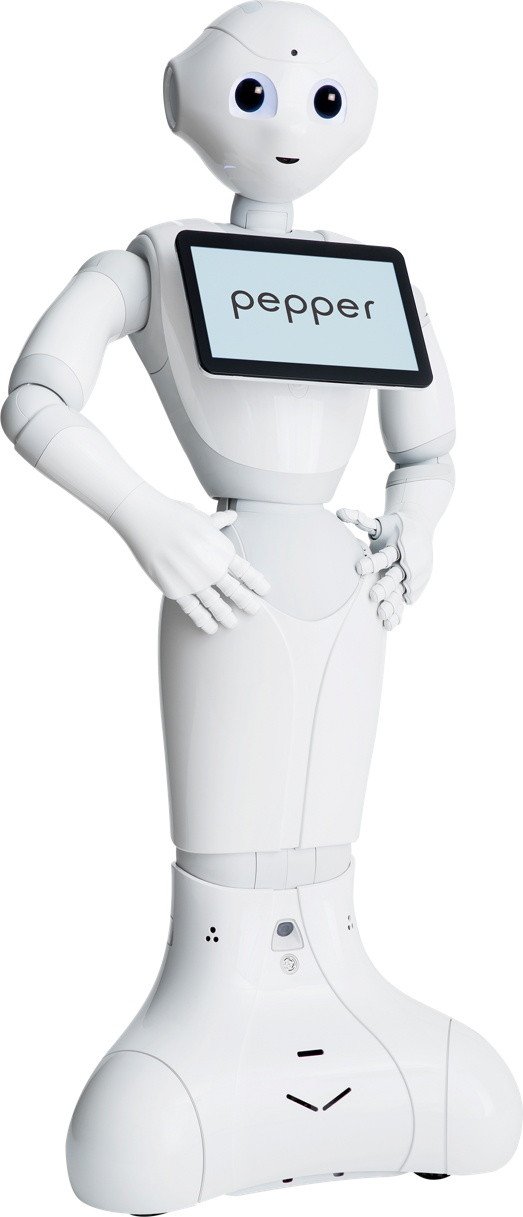
\includegraphics[scale=0.18]{img/pepper.png}
      \caption[The \textit{Pepper} robot]{
          The \textit{Pepper} robot\footnotemark
      }
\end{figure}
\footnotetext{
      Source:~\url{https://www.softbankrobotics.com/emea/themes/custom/softbank/images/full-pepper.png}
      (Accessed: 2020-03-30)
}

Since the \textit{Pepper} robot is highly customizable through software, it can be adapted for a wide
variety of scenarios. However, the lack of powerful or accurate arms limit it to mostly informational
roles. It is used as the platform for the \textit{RoboCup@Home Social Standard Platform League}~\
\cite{pepper-robot}.

Similarly, the \textit{Human Support Robot} by Toyota is used for the \textit{RoboCup@Home Domestic
Standard Platform League}. As the name suggests, these robots are supposed to assist humans in
domestic contexts and are not optimized for complex social interactions. They feature a simple
display for showing additional information~\cite{human-support-robot}.

Many teams in the \textit{RoboCup@Home Open Platform League 2019} also used various types of displays
for interfacing with their robots:

\begin{itemize}
    \item The \textit{CATIE Robotics} team uses modified PAL Robotics \textit{TIAGo} robots. The
          \textit{TIAGo} is equipped with a laptop tray that was customized to make it adjustable.
          An Android tablet was mounted to the back of the head to serve as a touch-capable input
          device~\cite{catie-robotics-tdp}.
    \item The \textit{homer@UniKoblenz} team also uses a \textit{TIAGo} as well as a custom robot based
          on the \textit{CU-2WD-Center} robot platform. It has a small head-mounted display that displays
          a face~\cite{homer-at-uni-koblenz-tdp}.
    \item The \textit{RoboFEI@Home} team uses a custom robot with an enclosure for an Apple iPad \SI{2}{"}
          tablet. The tablet is primarily used to display a face~\cite{robo-fei-at-home-tdp}.
    \item The \textit{RT Lions} team use a screen and a mini-beamer that projects images on a plastic
          dome to display the faces for their two robots~\cite{rt-lions-tdp}.
\end{itemize}

\chapter{Basics}
\label{basics}

This chapter explains some of the technologies used by the implementation. Section \ref{basics/rs-485}
and section \ref{basics/dynamixel-protocol} describe the bus and protocol used by the \textit{Wolfgang}
robot platform. Section \ref{basics/embedded-operating-systems} gives a brief overview of embedded
operating systems. The implementation uses an embedded OS to meet its latency requirements.

\section{RS-485}
\label{basics/rs-485}

\textit{RS-485} is a commonly used name for the ANSI TIA/EIA-485 standard. It is a specification for
a half duplex serial bus. Data is transmitted over two wires, usually labeled A and B, with a positive
voltage on A and a negative voltage on B. The voltage difference between these two wires determines
the actual logic level. A voltage difference less than or equal to \SI{-200}{\milli\volt} is a logical
0, while a difference greater than or equal to \SI{200}{\milli\volt} is a logical 1~\cite{rs-485-overview}.

This two wire setup makes the bus more resilient towards noise, allowing for operation in noisy
environments or over long distances.

For the purpose of this thesis the only interesting fact is the differential transmission. It requires
an additional transceiver to that converts the two signals into a single signal at the microcontroller's
logic level. Such a signal can then easily be consumed by a UART.

\section{ROBOTIS Dynamixel Protocol 2.0}
\label{basics/dynamixel-protocol}

The ROBOTIS Dynamixel Protocol is a packet based master/slave protocol used by all of ROBOTIS' products.
This section describes only the improved version 2.0. Official documentation can be found at ROBOTIS'
website~\cite{dynamixel-protocol-2}.

Each device is assigned a unique 8-bit ID that is used to determine the sender or receiver of packets.
IDs must be configured before connecting a device to the bus. The user must make sure that IDs do not
overlap. The IDs \lstinline{0xff} and \lstinline{0xfd} are not allowed and \lstinline{0xfe} is reserved
for broadcasts.

Once connected, the master (usually a powerful computer controlling the various devices) can send an
instruction packet. Instruction packets can target one or more devices (for details see
\ref{basics/dynamixel-protocol/instructions}). Only devices targeted by an instruction are allowed to
write a status packet to the bus. If an instruction targets more than one device, the responses are
ordered by their ID. Due to this, no external synchronization for the bus is required. Since instruction
or status packets may be lost, the master has to resend instruction packets if no packets have been
received after a certain amount of time.

Devices are seen as linear byte-addressed memory with 16-bit addresses (referred to as \textit{control tables}
by the official documentation). Usually these are memory-mapped registers that can be used to read or change
the state of a device. However, due to this simple view of a device as some amount of memory, the protocol can
be easily extended or reused by custom devices.

\begin{figure}[h]
    \centering

    \begin{subfigure}[t]{0.5\textwidth}
        \centering
        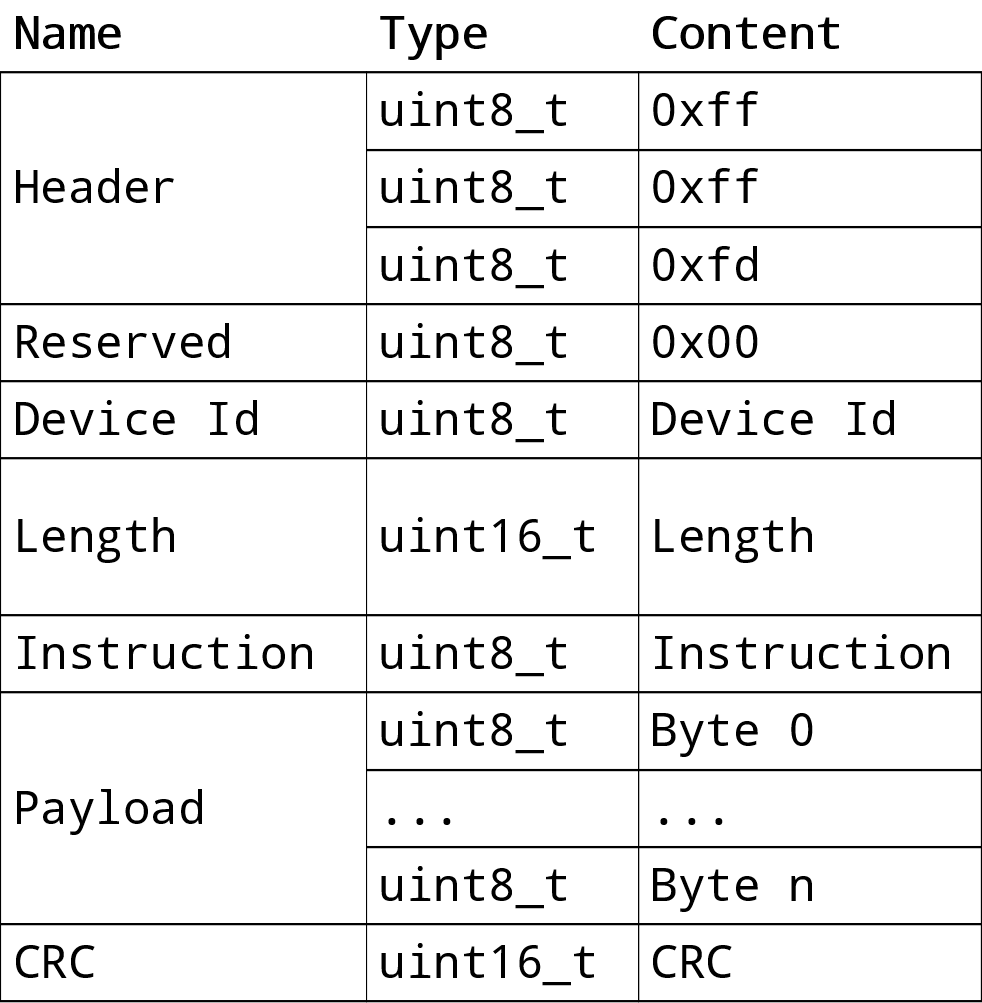
\includegraphics[scale=0.19]{img/packet.png}
        \caption{Generic layout of an instruction packet}
    \end{subfigure}%
    \begin{subfigure}[t]{0.5\textwidth}
        \centering
        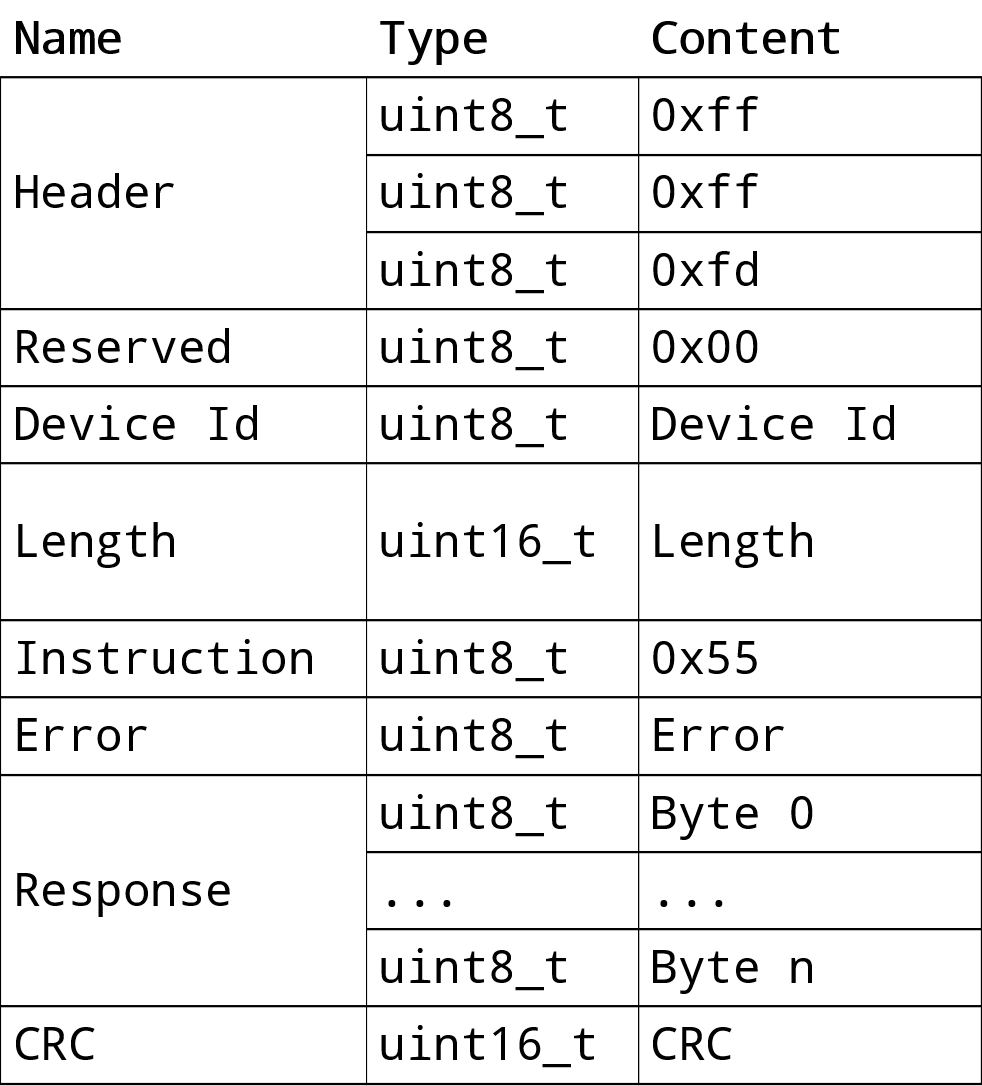
\includegraphics[scale=0.19]{img/status_packet.png}
        \caption{Generic layout of a status packet}
    \end{subfigure}

    \caption{Generic packet layout}
\end{figure}

Each packet has some metadata preceding the actual payload. It starts with a fixed byte sequence that allows
detecting a packet start without knowing where the last packet ended. It is followed by the device ID. For
instruction packets this is the device that is targeted, for status packets it is the device that sent the
packet. The \textit{Length} field determines the remaining length of the packet. This allows for a payload of variable
size, depending on the instruction used or the data returned by status packet. The next field is the instruction;
status packets use a reserved instruction. While the exact content of the payload varies, status packets always
store an additional error field as the first byte. This field can be used to indicate any errors that occurred
during processing of an instruction.

Since the payload can contain arbitrary values, it can also contain the byte sequence used to mark the start of
a new packet. To prevent a receiver from misinterpreting this byte sequence, \textit{byte stuffing} is used.
Whenever a payload contains the byte sequence \lstinline{0xff 0xff 0xfd}, it is replaced by
\lstinline{0xff 0xff 0xfd 0xfd}. This makes it impossible to send a payload that could be interpreted as the
start of a new packet. The receiver simply removes the extra byte that was added. Note that the
\textit{Length} field specifies the number of bytes with byte stuffing already applied.

The last two bytes of every packet contain the \textit{CRC-16/BUYPASS}~\cite{crc-16-buypass} checksum of
every byte in the packet, including the starting sequence (and excluding the CRC itself). This checksum
can be used to detect transmission errors, in case the underlying bus does not have error detection built
in (\textit{RS-485} does not).

\subsection{Instructions}
\label{basics/dynamixel-protocol/instructions}

\paragraph{Ping (\lstinline{0x01})}

Tests whether a device is connected. If the device ID is broadcast (\lstinline{0xfe}), all devices
respond. The status packet contains the device's model number and firmware version.

\begin{figure}[H]
    \centering
    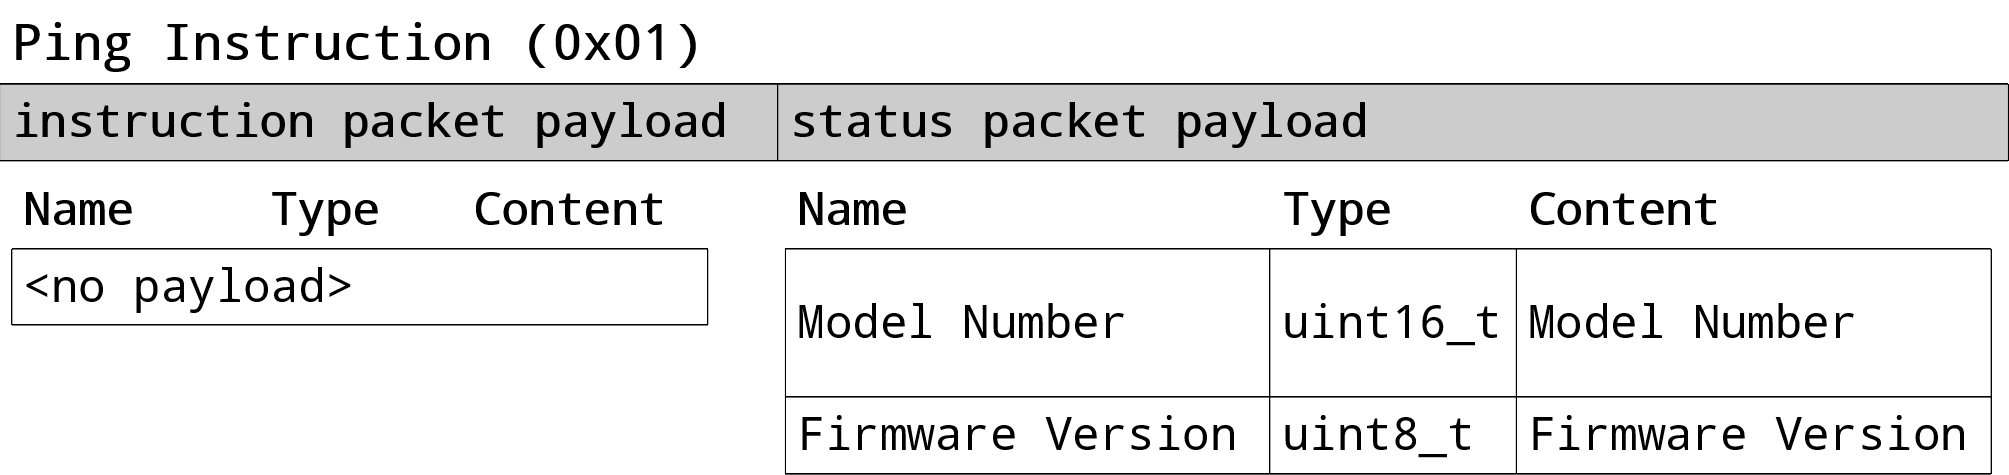
\includegraphics[scale=0.2]{img/ping_packet.png}
    \caption{\textit{Ping} instruction payloads}
\end{figure}

\paragraph{Read (\lstinline{0x02})}

Reads bytes from the \textit{control table} of a device. The status packet contains the requested
bytes.

\begin{figure}[H]
    \centering
    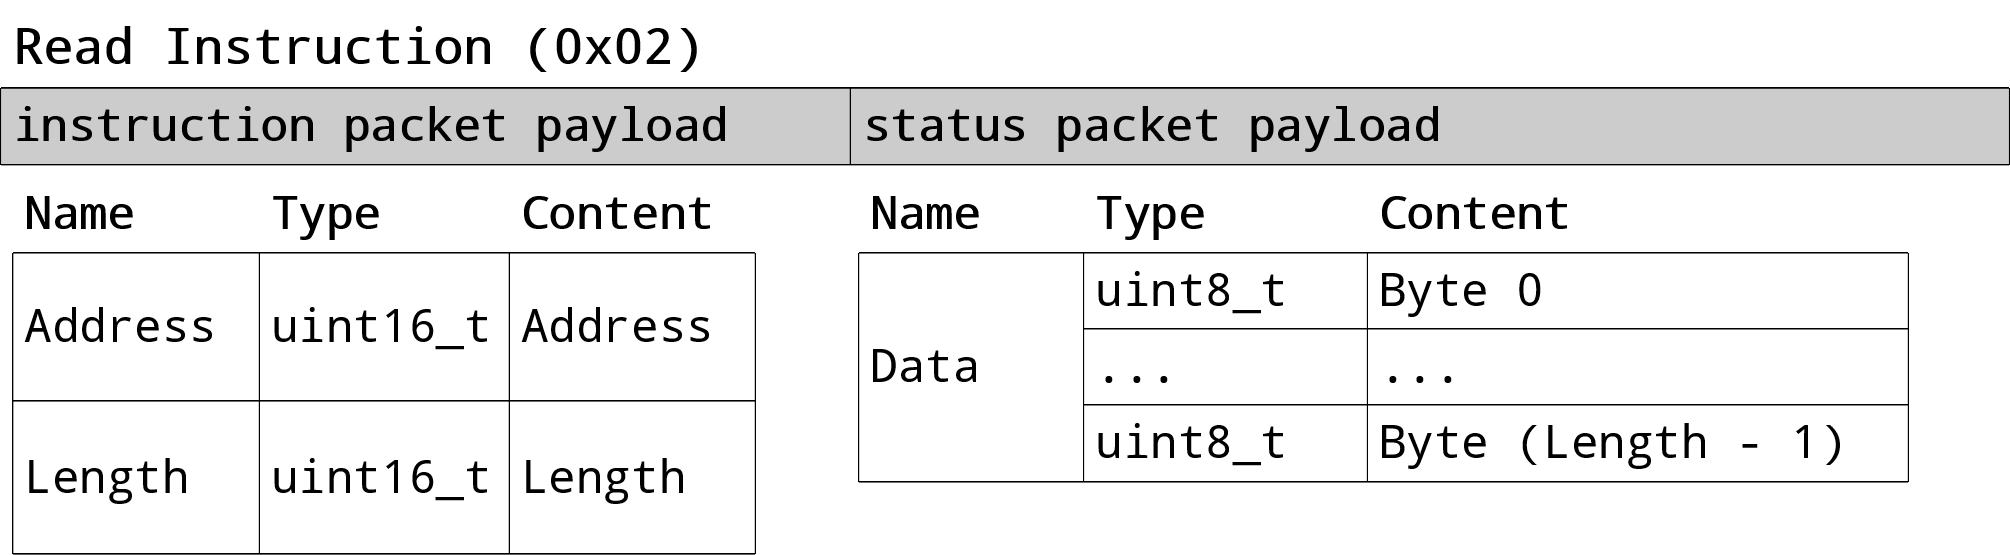
\includegraphics[scale=0.2]{img/read_packet.png}
    \caption{\textit{Read} instruction payloads}
\end{figure}

\paragraph{Write (\lstinline{0x03})}

Writes bytes to the \textit{control table} of a device. The status packet indicates whether the write
was executed successfully and contains no additional payload. Many devices can be configured to not
send any status packets on writes.

\begin{figure}[H]
    \centering
    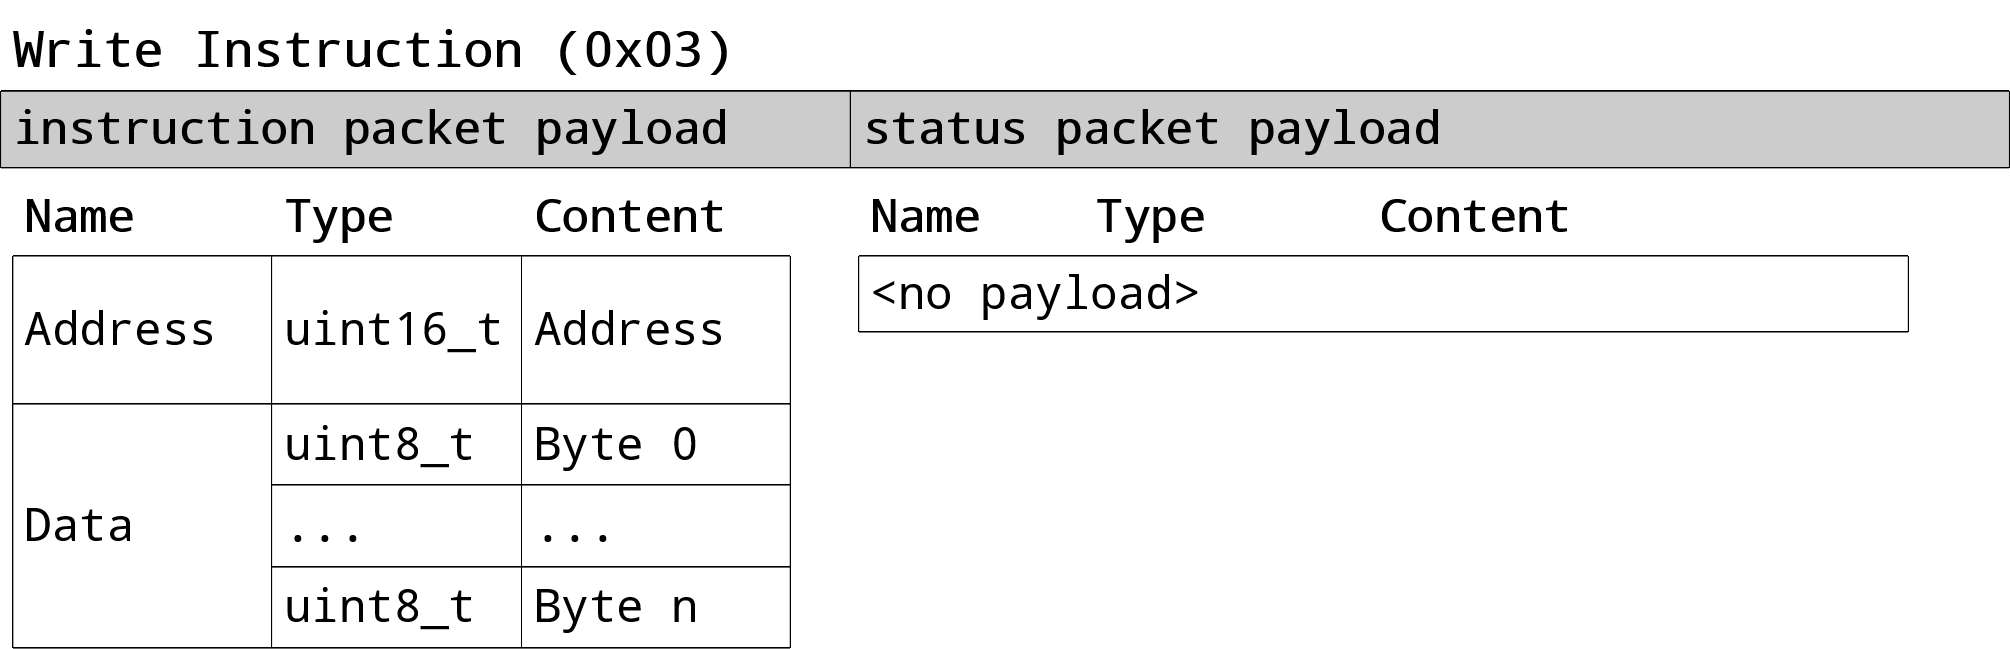
\includegraphics[scale=0.2]{img/write_packet.png}
    \caption{\textit{Write} instruction payloads}
\end{figure}

\paragraph{Reg Write (\lstinline{0x04})}

Identical to \textit{Write}, except that the write is delayed until an \textit{Action} instruction
is received.

\begin{figure}[H]
    \centering
    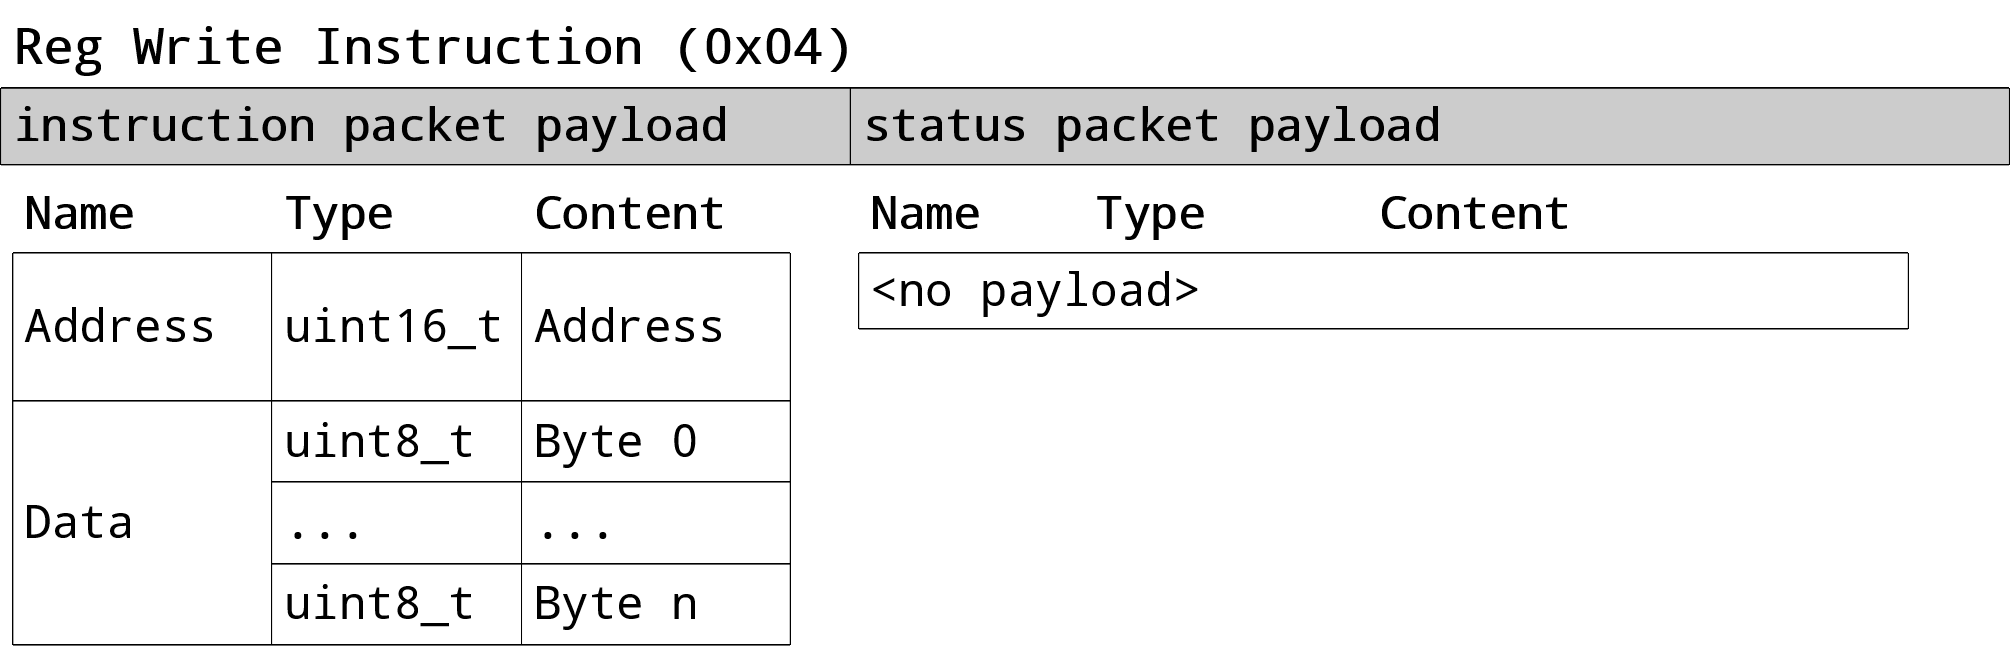
\includegraphics[scale=0.2]{img/reg_write_packet.png}
    \caption{\textit{Reg Write} instruction payloads}
\end{figure}

\paragraph{Action (\lstinline{0x05})}

Executes the write registered by the previous \textit{Reg Write} instruction. The status packet
indicates whether the write was executed successfully and contains no additional payload. Many
devices can be configured to not send any status packets on writes.

\begin{figure}[H]
    \centering
    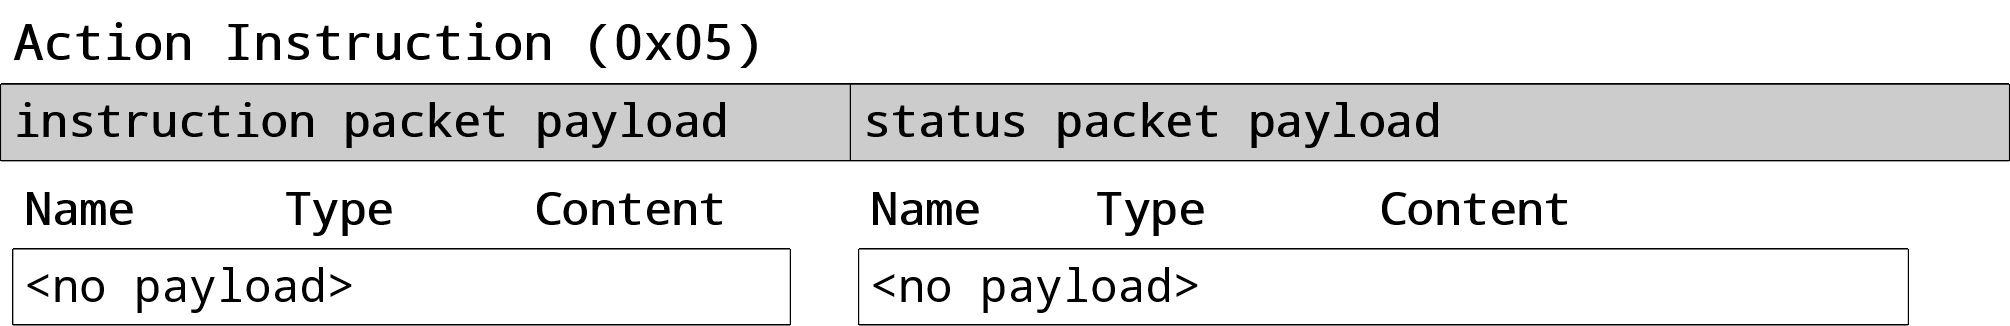
\includegraphics[scale=0.2]{img/action_packet.png}
    \caption{\textit{Action} instruction payloads}
\end{figure}

\paragraph{Factory Reset (\lstinline{0x06})}

Resets the device's \textit{control table} fields to their default values. \textit{Reset Mode}
determines the values that are reset:

\begin{itemize}
    \item \lstinline{0xff}: resets all values
    \item \lstinline{0x01}: resets all values except for the ID
    \item \lstinline{0x02}: resets all values except for the ID and the baud rate
\end{itemize}

The status packet indicates whether the reset was executed successfully and contains no additional
payload.

\begin{figure}[H]
    \centering
    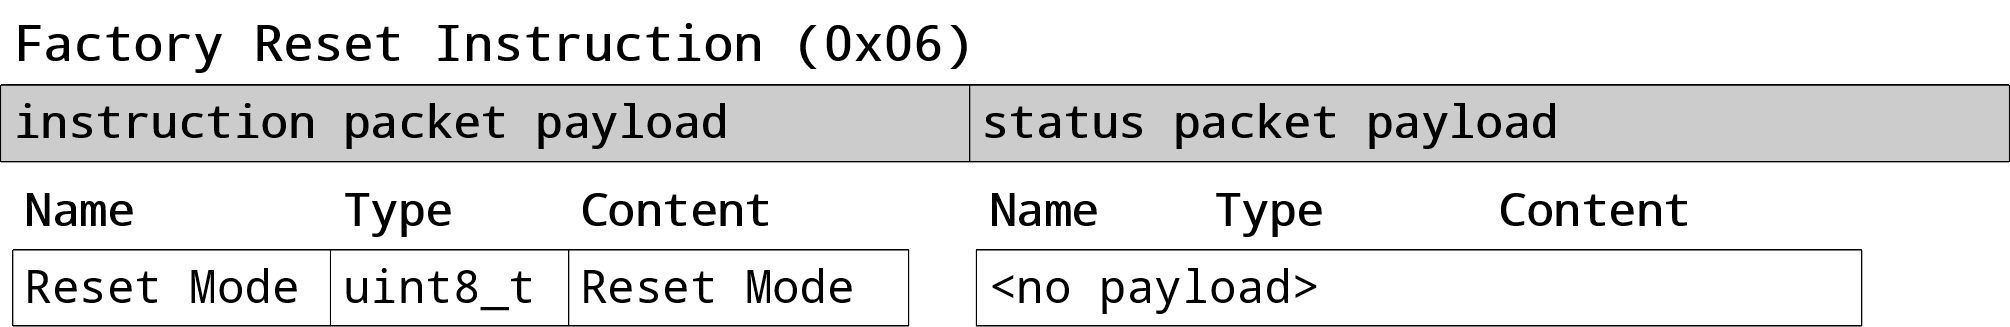
\includegraphics[scale=0.2]{img/factory_reset_packet.png}
    \caption{\textit{Factory Reset} instruction payloads}
\end{figure}

\paragraph{Reboot (\lstinline{0x08})}

Reboots the device. The status packet indicates whether the reboot was successful and contains no
additional payload.

\begin{figure}[H]
    \centering
    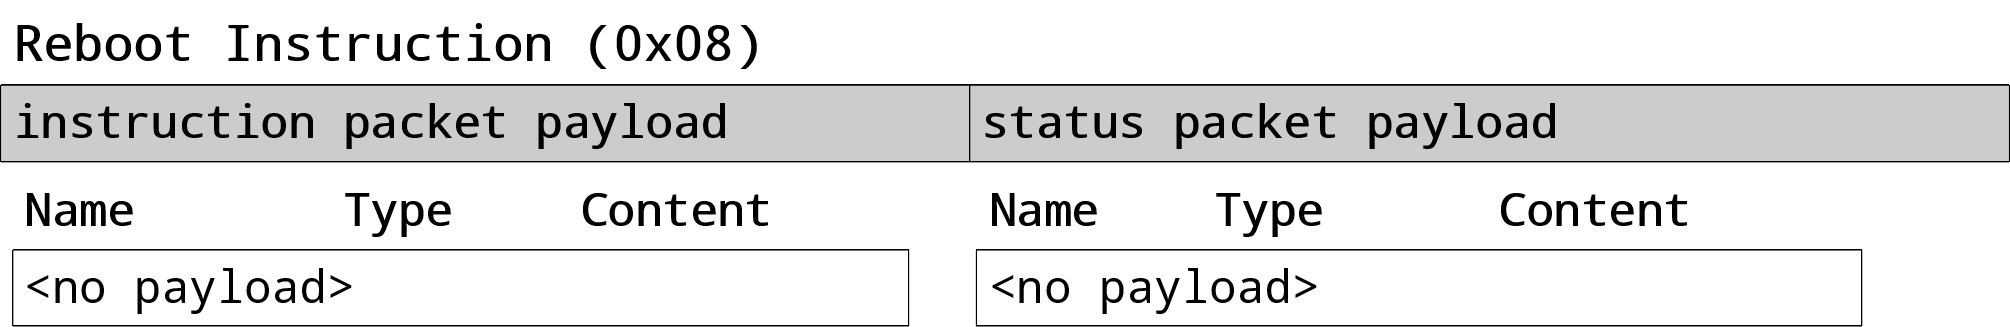
\includegraphics[scale=0.2]{img/reboot_packet.png}
    \caption{\textit{Reboot} instruction payloads}
\end{figure}

\paragraph{Clear (\lstinline{0x10})}

Resets the multi turn information of the device. This instruction is very closely tied to servos
and generally not useful for other kinds of devices.

\begin{figure}[H]
    \centering
    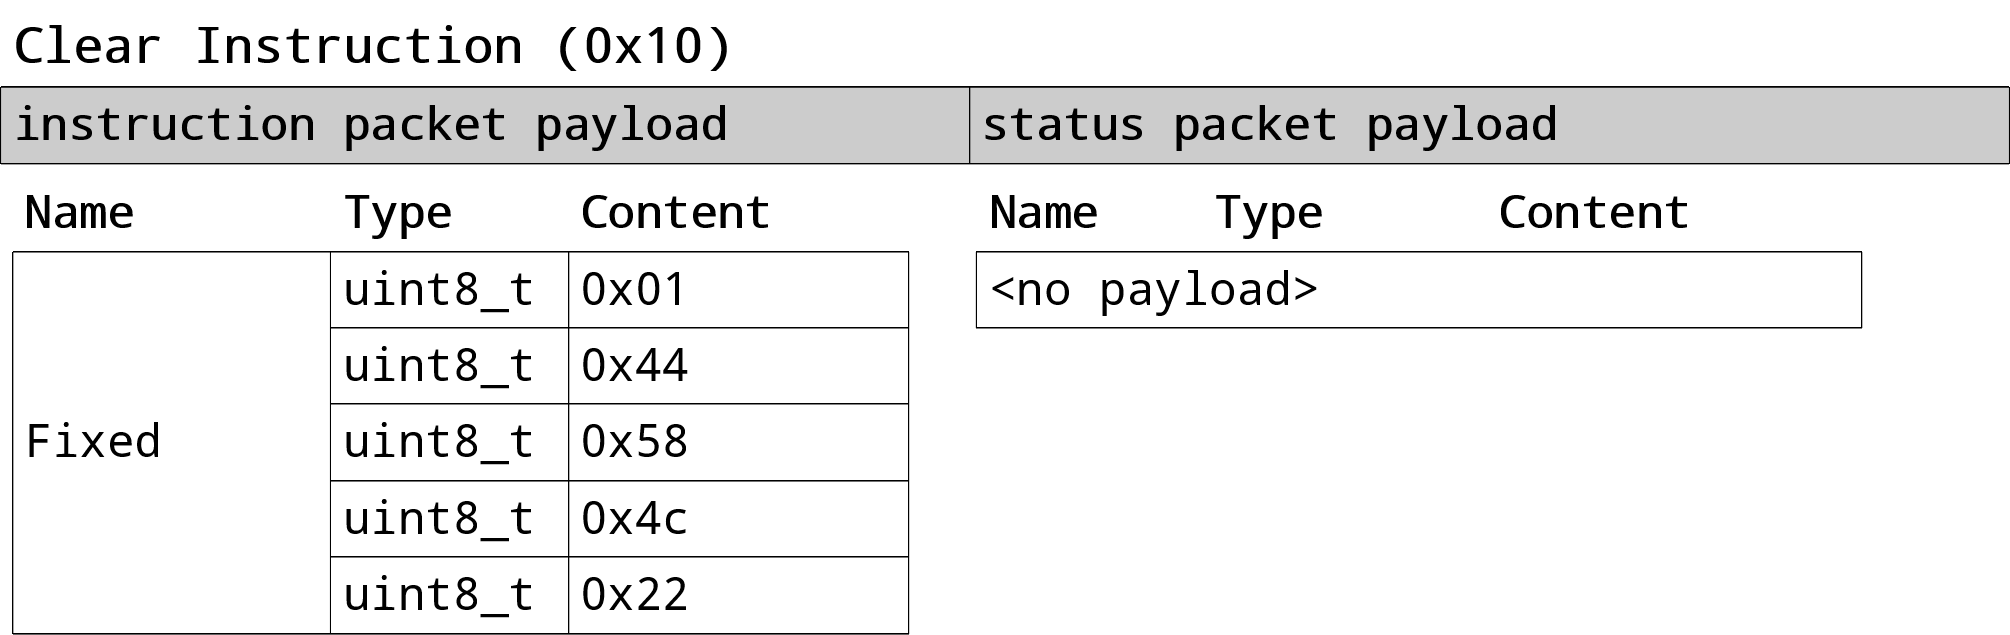
\includegraphics[scale=0.2]{img/clear_packet.png}
    \caption{\textit{Clear} instruction payloads}
\end{figure}

\paragraph{Sync Read (\lstinline{0x82})}

Reads bytes from the \textit{control tables} of multiple devices at once. The device ID of the
instruction packet must be broadcast (\lstinline{0xfe}). The status packet of each device contains
the requested bytes. Devices respond in the same order as the their IDs in the instruction packet
payload.

\begin{figure}[H]
    \centering
    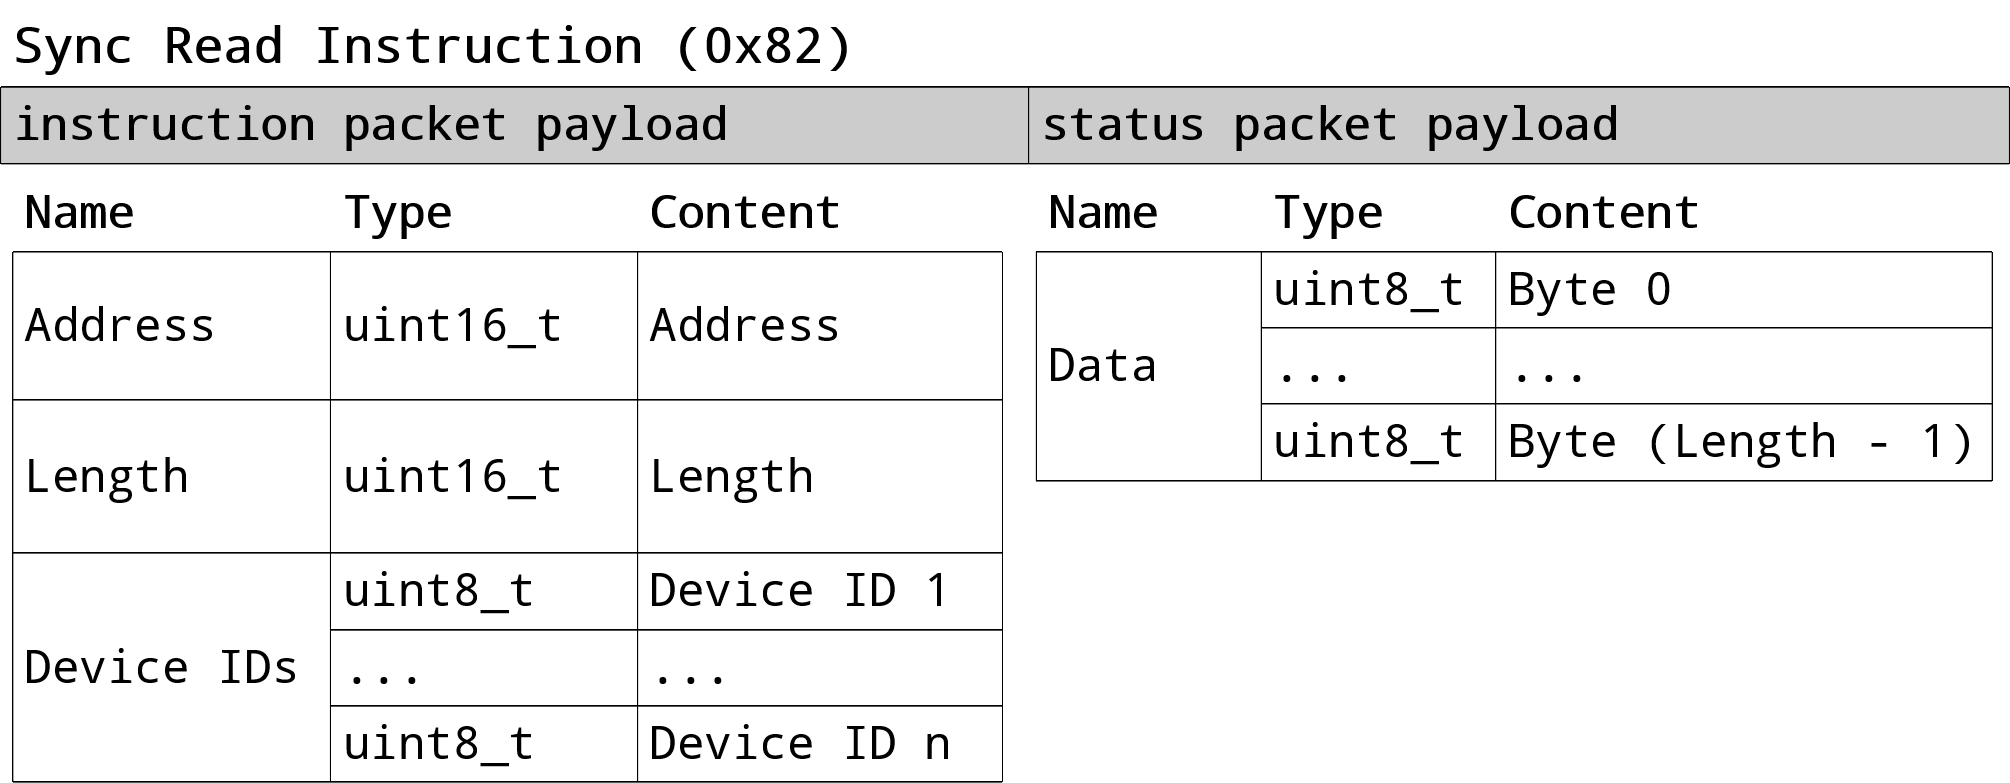
\includegraphics[scale=0.2]{img/sync_read_packet.png}
    \caption{\textit{Sync Read} instruction payloads}
\end{figure}

\paragraph{Sync Write (\lstinline{0x83})}

Writes bytes to the \textit{control tables} of multiple devices at once. The data for each device
can be different. The device ID of the instruction packet must be broadcast (\lstinline{0xfe}). The
status packet of each device indicates whether the write was executed successfully and contains no
additional payload. Devices respond in the same order as the their IDs in the instruction packet
payload. Many devices can be configured to not send any status packets on writes.

\begin{figure}[H]
    \centering
    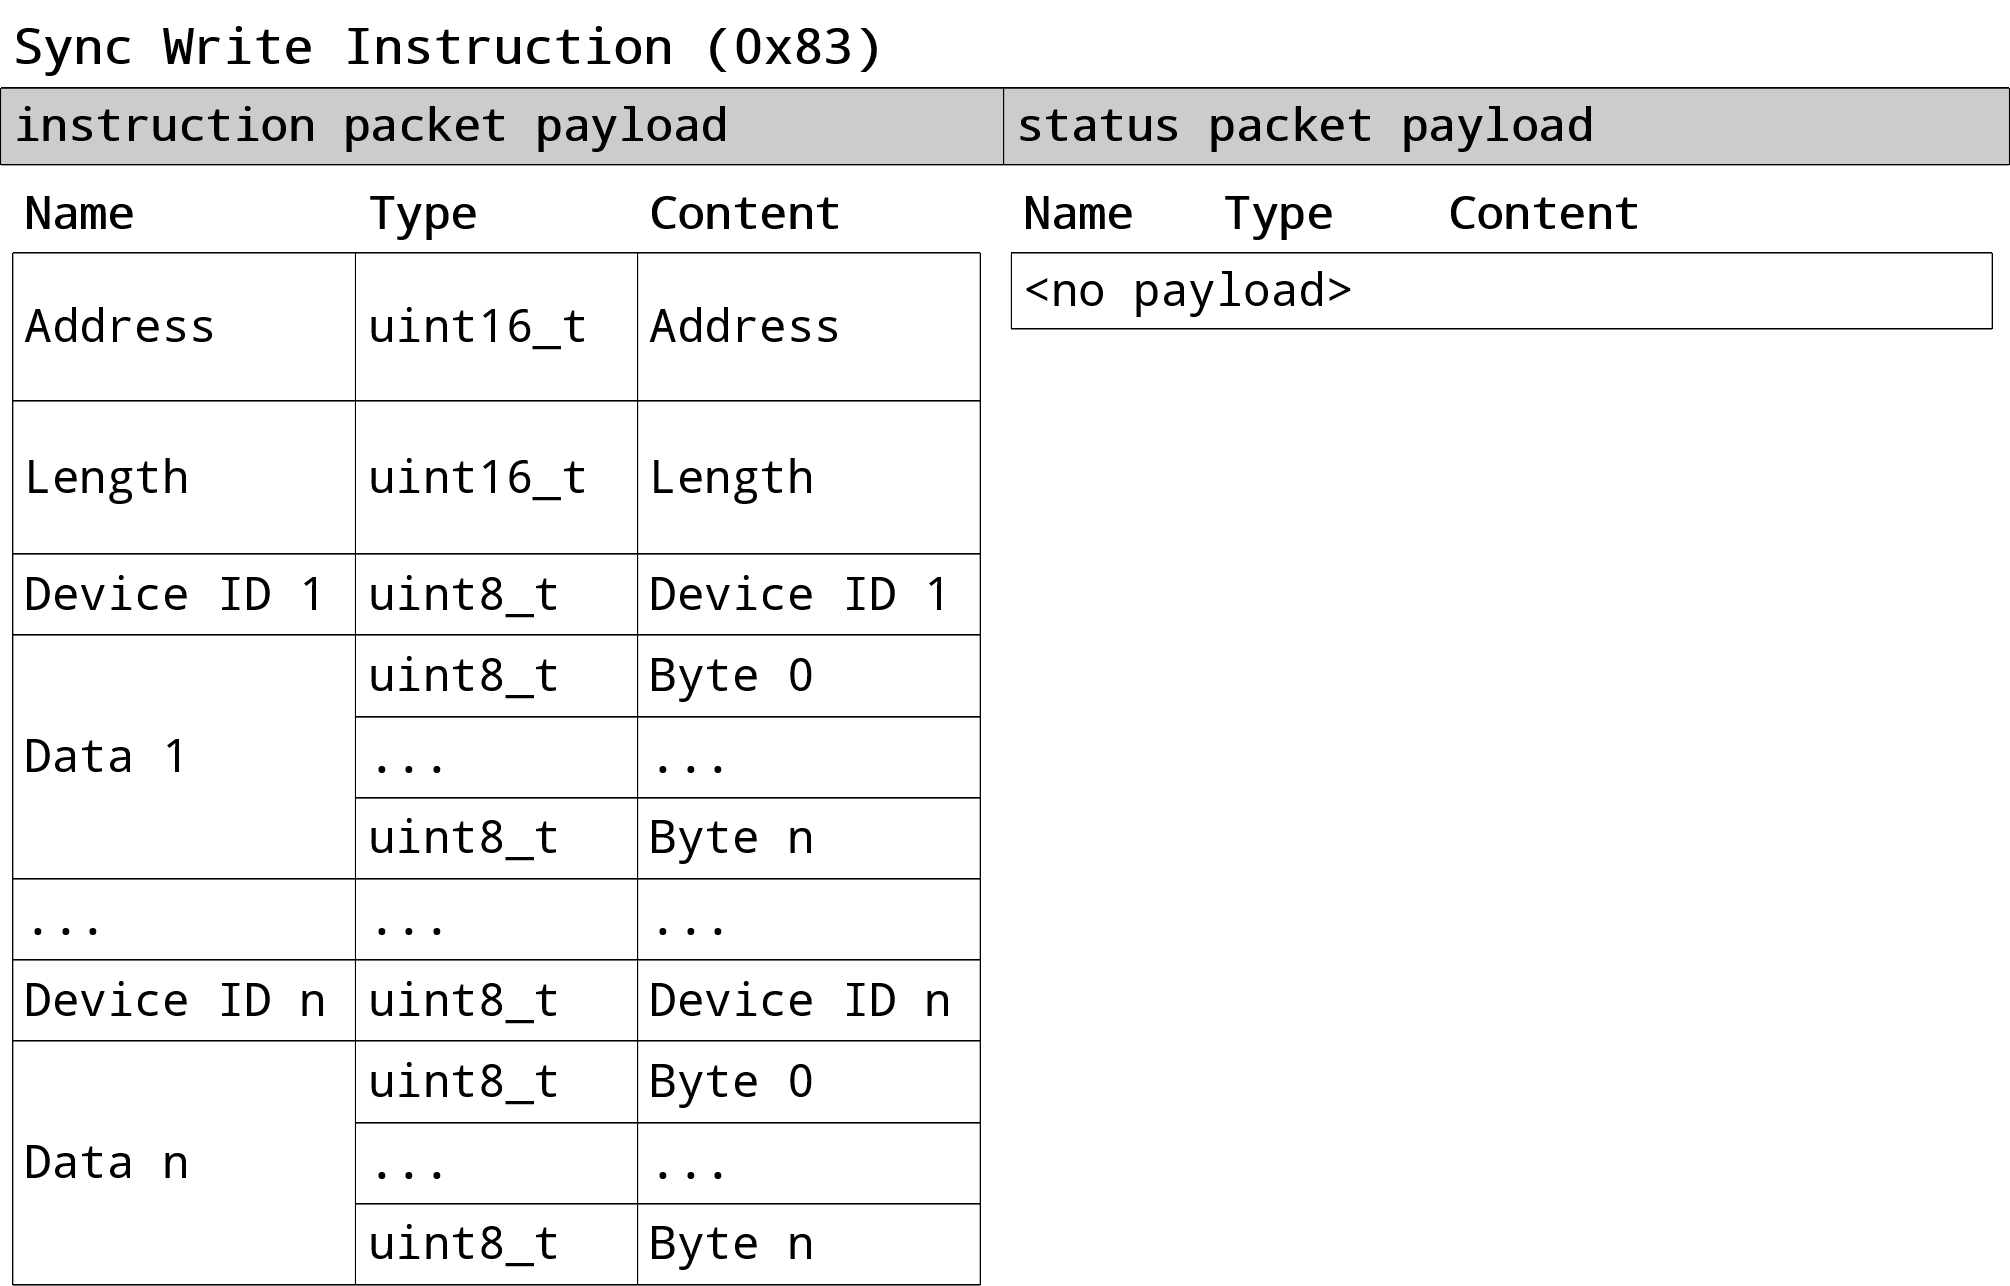
\includegraphics[scale=0.2]{img/sync_write_packet.png}
    \caption{\textit{Sync Write} instruction payloads}
\end{figure}

\paragraph{Bulk Read (\lstinline{0x92})}

Reads bytes from the \textit{control tables} of multiple devices at once. Unlike \textit{Sync Read},
this instruction allows for different addresses and lengths for each device. The device ID of the
instruction packet must be broadcast (\lstinline{0xfe}). The status packet of each device contains
the requested bytes. Devices respond in the same order as the their IDs in the instruction packet
payload.

\begin{figure}[H]
    \centering
    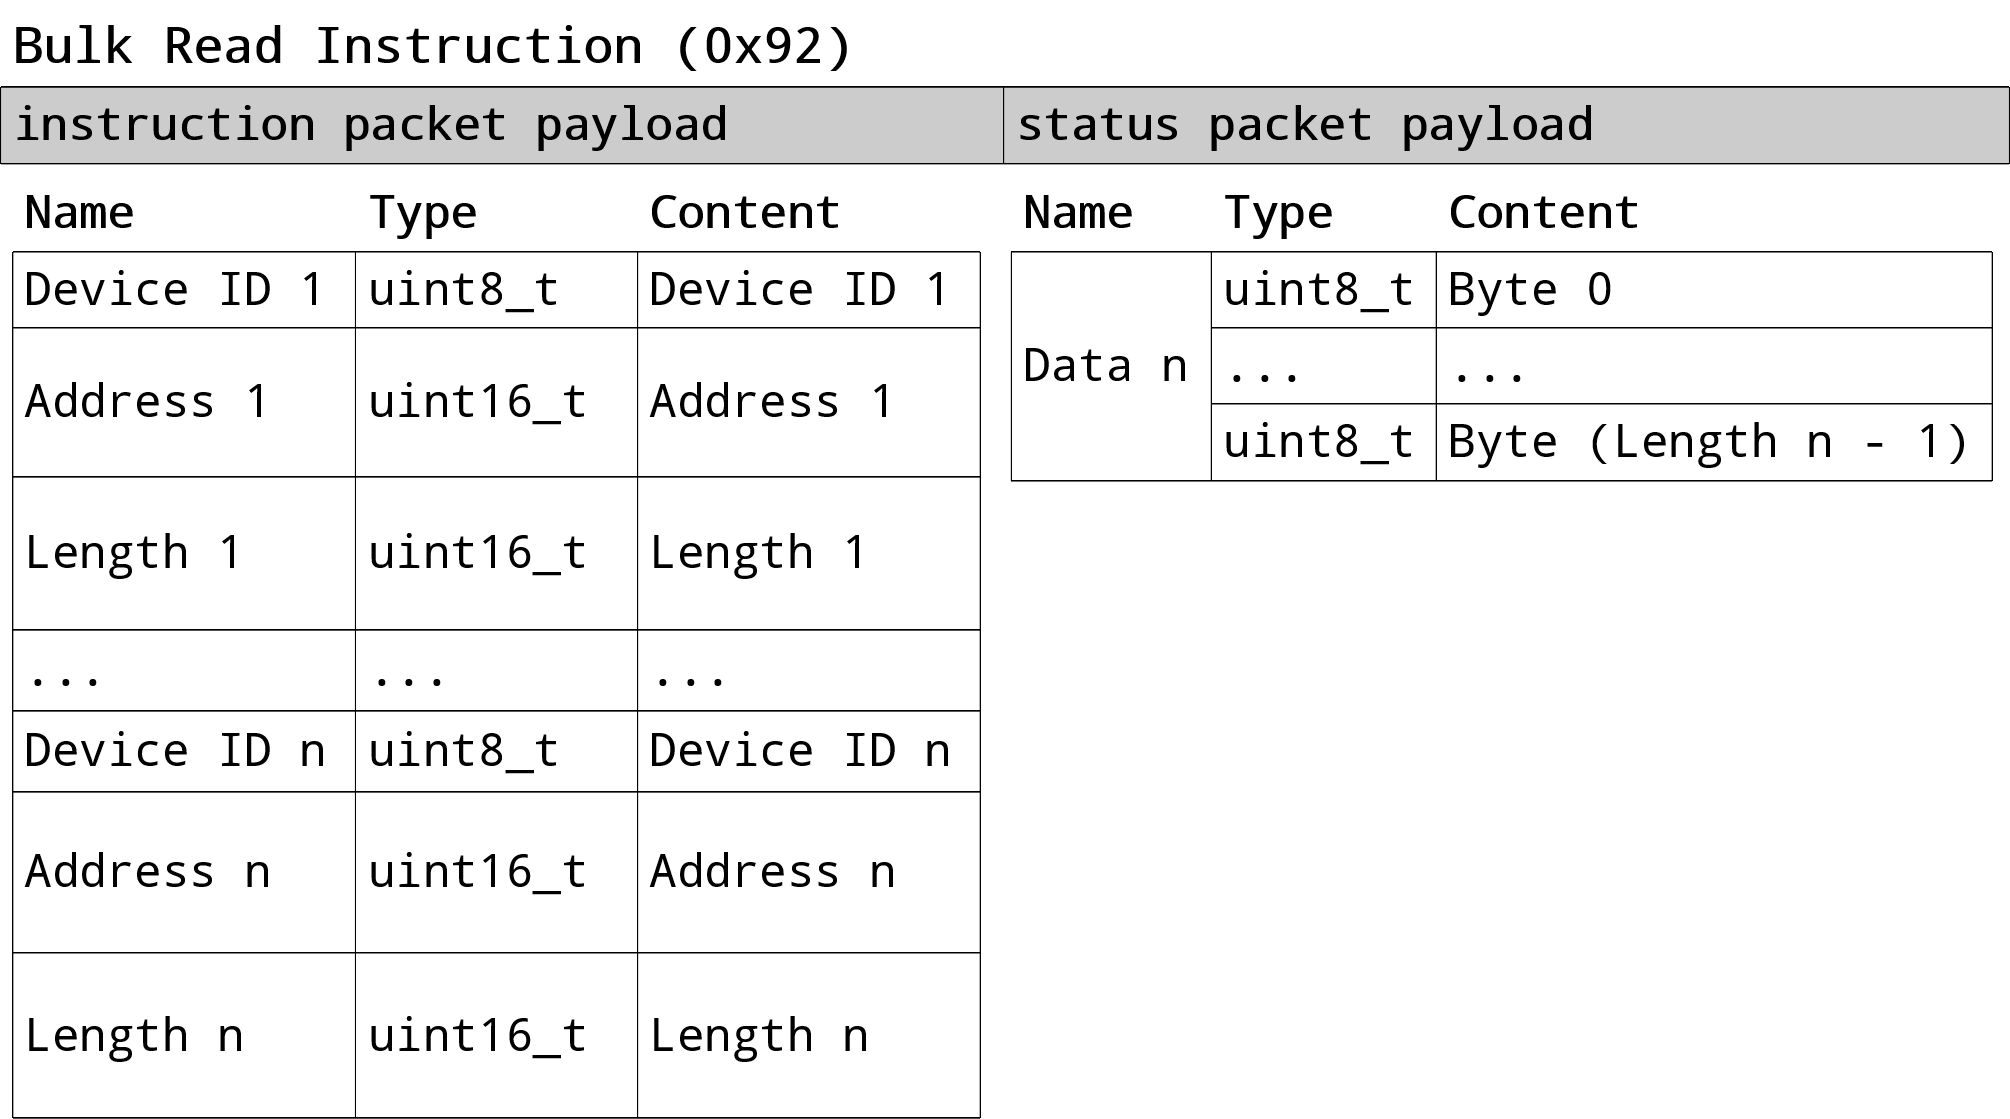
\includegraphics[scale=0.2]{img/bulk_read_packet.png}
    \caption{\textit{Bulk Read} instruction payloads}
\end{figure}

\paragraph{Bulk Write (\lstinline{0x93})}

Writes bytes to the \textit{control tables} of multiple devices at once. Unlike \textit{Sync Write},
this instruction allows not only for different data but also for different addresses and lengths for
each device. The device ID of the instruction packet must be broadcast (\lstinline{0xfe}). The status
packet of each device indicates whether the write was executed successfully and contains no additional
payload. Devices respond in the same order as the their IDs in the instruction packet payload. Many
devices can be configured to not send any status packets on writes.

\begin{figure}[H]
    \centering
    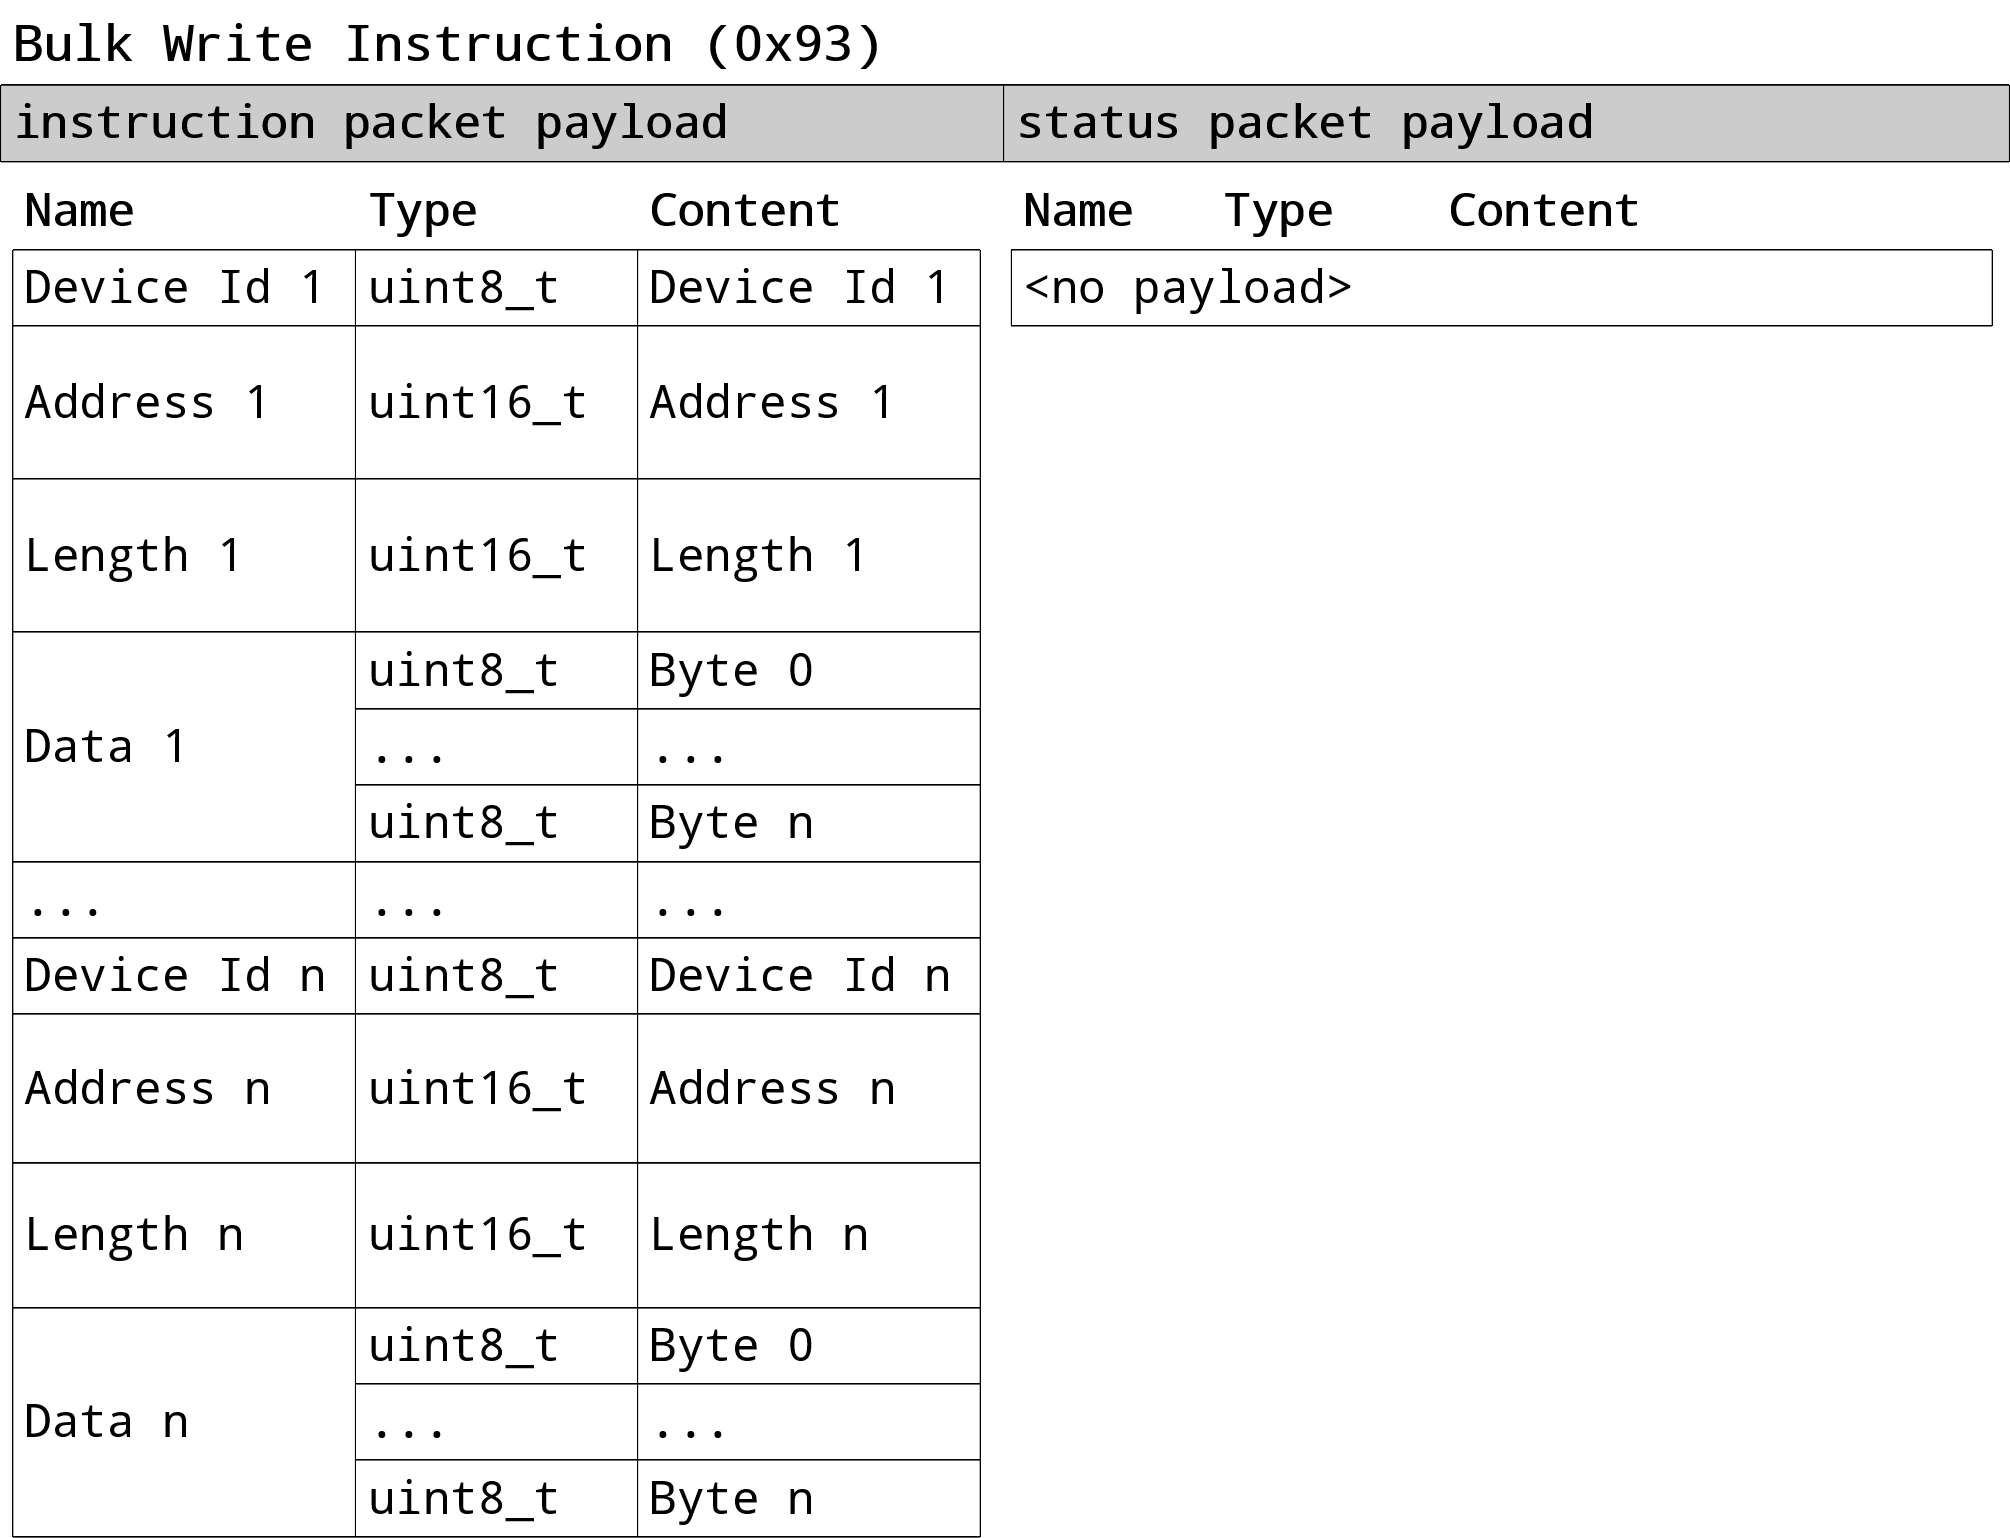
\includegraphics[scale=0.2]{img/bulk_write_packet.png}
    \caption{\textit{Bulk Write} instruction payloads}
\end{figure}

\subsection{Byte-Order}
\label{basics/dynamixel-protocol/byte-order}

All multi-byte values (packet fields, values in packet payloads and \textit{control table} fields) are
\textit{little-endian}. That is, for multi-byte values, the least significant byte comes first, then the
second least significant byte, etc.

\section{Embedded Operating Systems}
\label{basics/embedded-operating-systems}

Embedded operating systems are libraries linked directly with the user's code. They are small
both in runtime overhead and in program size, making them ideal for microcontrollers that cannot run
full operating systems like Linux or Windows. Embedded OSs only provide a small subset of the many
features offered by traditional operating systems. Common features are:

\begin{itemize}
    \item threads (sometimes also called tasks)
    \item concurrency primitives (mutexes, semaphores, queues, etc)
    \item memory allocators
    \item file systems
\end{itemize}

The most significant difference to traditional operating systems is the lack of security. Since the
operating system is part of the program itself, all code can be trusted and process boundaries are
not needed~\cite{modern-os-embedded-os}.

The core of an embedded OS are threads and context switching. Being part of the user program, the
application must configure an interrupt that calls the scheduler, which in turn runs application
code in one of the threads. Threads can run on separate CPU cores but they are also useful on single
core systems. Threads are preemptive: one thread can be paused and another one started instead. This
makes it possible to guarantee that some threads always get the CPU time they need, for example to
process incoming data~\cite{freertos-fundamentals}.

The concurrent nature of threads makes it necessary to synchronize access to shared data. Since
synchronization is deeply intertwined with the scheduler, concurrency primitives must also be
provided by the embedded OS.

\chapter{Implementation}
\label{implementation}

This chapter describes the hardware the implementation uses (section \ref{implementation/hardware})
and the developed firmware (section \ref{implementation/software}). The source code for the firmware
can be found at \url{https://github.com/Laegluin/embedded_debug_interface_for_robots/tree/thesis-ref}.
The version referenced by this thesis is tagged as \lstinline{thesis-ref}. The description of the
firmware is intended to give a high level overview and discusses tradeoffs as well as points of
interest.

Since the implementation targets the \textit{Wolfgang} robot platform, it must be compatible with
its \textit{RS-485} bus running at a speed of \SI{2}{\mega{Bd}}.

\section{Hardware}
\label{implementation/hardware}

The following hardware is used:

\begin{itemize}
    \item STM32F7508-DK development board\footnote{\url{https://www.st.com/resource/en/user_manual/dm00537062-discovery-kit-for-stm32f7-series-with-stm32f750n8-mcu-stmicroelectronics.pdf}}
    \item MAX485 RS-485/RS-422 transceiver\footnote{\url{https://datasheets.maximintegrated.com/en/ds/MAX1487-MAX491.pdf}}
    \item FT232R USB to UART converter (for testing)\footnote{\url{https://www.ftdichip.com/Support/Documents/DataSheets/ICs/DS_FT232R.pdf}}
\end{itemize}

The MAX485 transceiver is used to connect the \textit{RS-485} bus to the STM32F7508-DK board. It
outputs a \SI{5}{\volt} signal that can be interpreted by one of the board's UARTs. STM32F7508-DK
is built around a STM32F750N8H6 Arm Cortex-M7 based microcontroller. The controller's \textit{UART6}
is used, as it is easily accessible through the board's Arduino Uno compatible connectors at the
back. All UARTs have a theoretical maximum speed of \SI{27}{\mega{Bd}}~\cite{mcu-ref-manual} (depending
on the clock configuration), making the MAX485's maximum speed of \SI{2.5}{\mega{Bd}} the maximum speed
of this setup~\cite{max-485-manual}\cite{board-user-manual}.

The STM32F7508-DK board has a built in \SI{4.3}{"} 480x272 LCD-TFT capacitive touchscreen. It is
used to display and interact with the UI. Because it is built in, no further assembly is required~\
\cite{board-user-manual}.

The STM32F750N8H6 microcontroller is based on an Arm Cortex-M7 CPU. It supports clock speeds of up to
\SI{216}{\mega\hertz} and has both data and instruction caches. It is equipped with a single-precision
FPU (floating point unit) and a DMA controller~\cite{mcu-datasheet}. While this is quite a lot of
processing power for a microcontroller, it is needed to drive an interactive UI while at the same time
processing incoming data quickly enough. The DMA controller allows transferring data from the UART to
memory at high data rates without using up CPU time.

The controller itself comes with only \SI{64}{KiB} of embedded flash memory. However, it also has a
Quad-SPI memory interface that can be used with external flash memory~\cite{mcu-datasheet}. The
STM32F7508-DK board has \SI{16}{MiB} of pre-installed flash memory~\cite{board-user-manual}.

Similarly, \SI{320}{KiB} of RAM are embedded in controller~\cite{mcu-datasheet}. This is more than
enough for most applications but not enough for the video RAM (VRAM) used by the display. When using
double buffering and 8 bits per pixel, at least $480 \cdot 272 \cdot 3 \cdot 2 = 765\,\si{KiB}$ are
needed for VRAM alone. VRAM can be located in external RAM which can be controlled by the microcontroller's
FMC (flexible memory controller). The board has \SI{8}{MiB} of pre-installed external RAM~\
\cite{mcu-datasheet}\cite{board-user-manual}.

The STM32F7508-DK board is equipped with an ST-LINK/V2-1 in-circuit debugger. It can be used for
debugging and for programming the internal flash memory~\cite{board-user-manual}. External flash
cannot be programmed using the ST-LINK; instead a standalone bootloader must be used (see subsection
\ref{implementation/software/bootloader}).

The FT232R USB to UART converter is only used for testing and benchmarking. It can easily be connected
to \textit{UART6} instead of the MAX485. Data can then be sent to the USB serial port emulated by
the FT232R from the computer connected to it~\cite{ftdi-232r-datasheet}. This makes testing extremely
easy since the device can be treated as a serial terminal.

\section{Software}
\label{implementation/software}

This section describes the firmware for the STM32F7508-DK board. The bootloader is written in C
(C99), the actual firmware itself is written in C++ (C++14). All code is compiled with the
\textit{GNU arm-none-eabi} toolchain. \textit{Newlib} is used as the C standard library implementation.

\subsection{Bootloader}
\label{implementation/software/bootloader}

When the microcontroller is reset, it loads the \textit{vector table} from address \mbox{\lstinline{0x00000000}.}
The \textit{vector table} contains the addresses of all possible interrupt handlers. In addition, the
first item is the initial value of the stackpointer and the second is the address of the entry point.
After loading the \textit{vector table}, the stackpointer is set to the configured value and the
processor jumps to the entry point~\cite{mcu-ref-manual}. By default, addresses in the range
\lstinline{[0x00000000, 0x08000000)} are mapped to \lstinline{0x08000000}, which in turn is mapped
to internal flash memory~\cite{mcu-ref-manual}.

This poses a problem for applications that do not fit into internal flash memory: there is no way to
boot from the much larger Quad-SPI flash memory or to program it. An additional bootloader has to be
used instead. A bootloader is a minimal application that initializes a peripheral device for I/O,
accepts commands as well as data from said device and allows programming and booting from otherwise
unsupported memory.

In this case, the bootloader must allow programming and booting from Quad-SPI flash memory. It uses
one of the STM32F7508-DK board's micro-USB ports for I/O~\cite{board-user-manual}. USB is a well
suited interface because data integrity checks are built in~\cite{usb-2-spec}. STMicroelectronics
provides a USB 2.0 compliant library for applicable microcontrollers that the bootloader uses for
USB support~\cite{stm32-usb-lib}.

When the bootloader starts, it initializes the USB controller and the Quad-SPI memory interface. It
also blinks the board's LED at regular intervals to indicate that it is running. It then listens on
the USB interface as a communication class device.

\begin{figure}[h]
    \centering

    \begin{subfigure}[t]{0.5\textwidth}
        \centering
        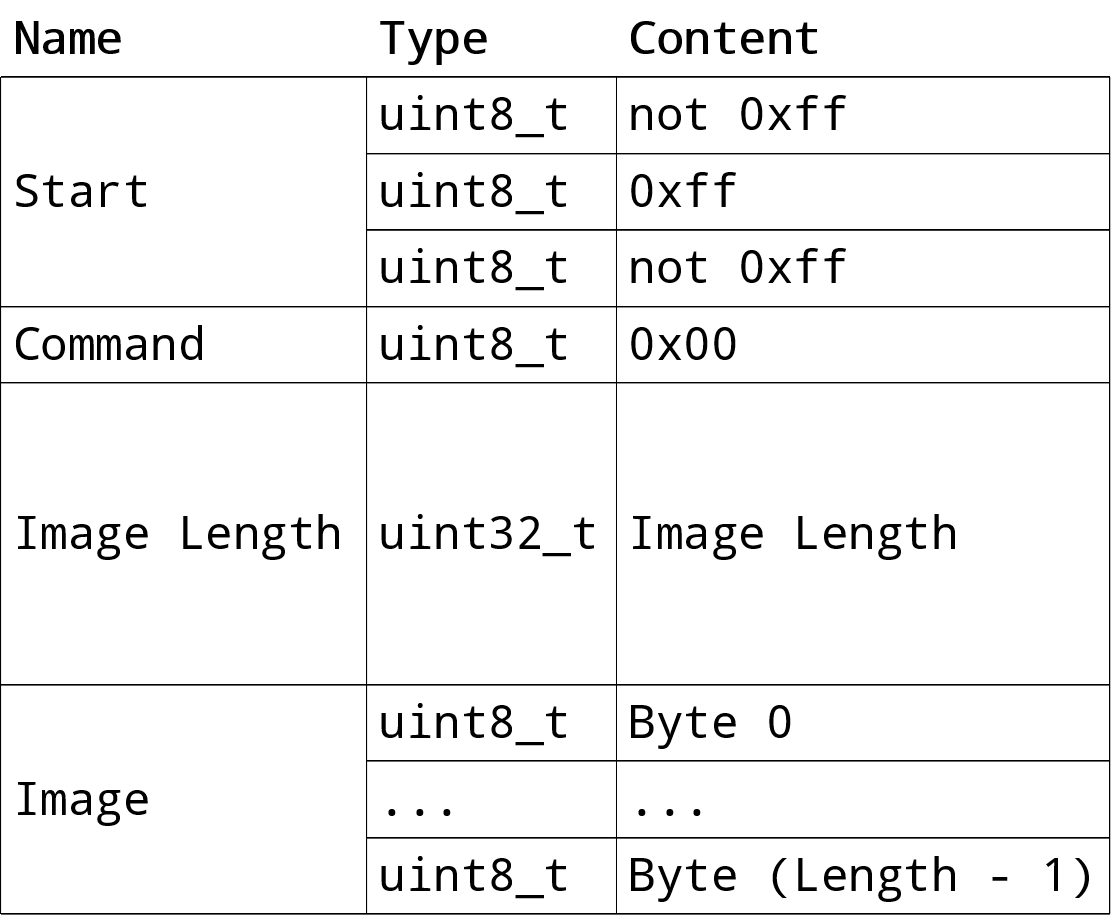
\includegraphics[scale=0.18]{img/bootloader_flash_packet.png}
        \caption{\textit{flash} packet layout}
    \end{subfigure}%
    \begin{subfigure}[t]{0.5\textwidth}
        \centering
        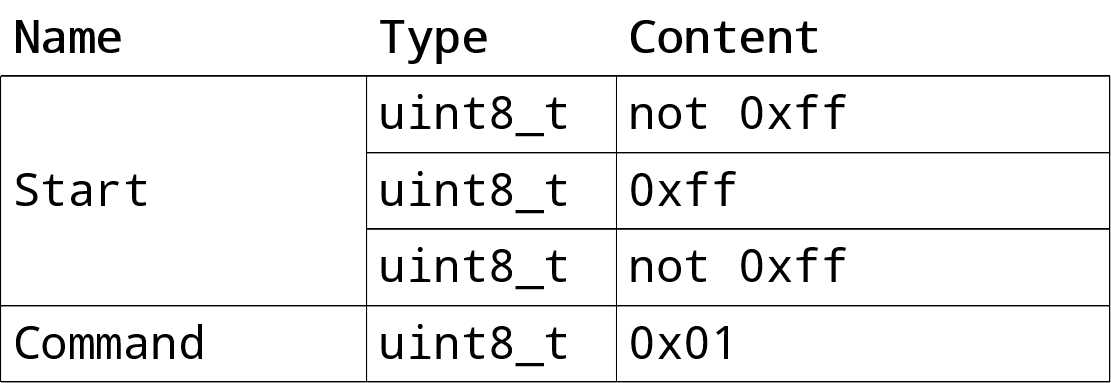
\includegraphics[scale=0.18]{img/bootloader_start_packet.png}
        \caption{\textit{start} packet layout}
    \end{subfigure}

    \caption{Bootloader packet layout}
    \label{implementation/software/bootloader/packet-layout}
\end{figure}

The bytes received are interpreted according to a custom, packet based protocol. The packet layout
can be seen in figure \ref{implementation/software/bootloader/packet-layout}. Packets start with a
start sequence that makes it possible to identify the beginning of a packet even if it is preceded
by unrelated bytes. To prevent unwanted start sequences in the packet itself, all bytes following
the start sequence must be escaped by adding \textit{byte stuffing}: whenever a byte that is not
\lstinline{0xff} is followed by a \lstinline{0xff} byte, another \lstinline{0xff} byte must be added.
For example, the bytes \lstinline{0x00 0xff 0xff} must be sent as \lstinline{0x00 0xff 0xff 0xff}.
The bootloader simply removes the added bytes before processing the rest. Values of more than one
byte are encoded as \textit{little-endian} and lengths are always given as the length before any
\textit{byte stuffing} was applied.

A \textit{flash} packet instructs the bootloader to erase and then program the Quad-SPI flash memory
with all the bytes in the \textit{Image} field, beginning at the start address of the Quad-SPI flash
memory.

\begin{figure}[h]
    \centering
    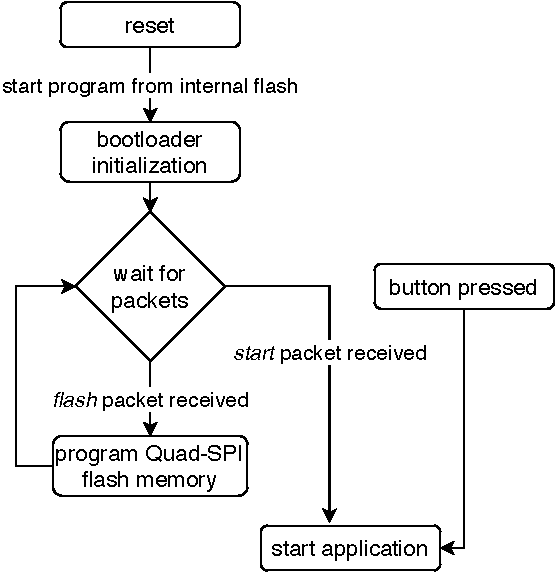
\includegraphics[scale=1.0]{img/bootloader_flowchart.pdf}
    \caption[Bootloader program flow]{
        After reset, the microcontroller starts the program in internal flash memory (the bootloader).
        It then waits for packets to arrive over USB. If a \textit{start} packet has been received or
        the button was pressed, it starts the application in Quad-SPI flash memory.
    }
\end{figure}

The \textit{start} packet instructs the bootloader to start an application previously flashed. It
disables all (pending) interrupts, exits interrupt handler mode if necessary and enables the
memory-mapped mode for the Quad-SPI memory interface. In addition it also enables the board's LED
permanently, indicating that the application is now running. Finally, it starts the application by
loading the stackpointer and jumping to the entry point in the same way the microcontroller does
when it boots from internal flash memory. The bootloader assumes that the application's \textit{vector table}
starts at the beginning of the Quad-SPI flash memory space (\lstinline{0x90000000}~\cite{mcu-ref-manual}).
The application can also be started by pressing the board's programmable button (next to the reset
button). The procedure is identical to the one described above.

The bootloader only has to be flashed to internal flash memory once. Afterwards, it can be used to
program the Quad-SPI flash memory and start an application from it using the board's micro-USB port.
In this case, the application is the actual firmware that controls the UI and processes packets
sent over the \textit{Wolfgang} robot platform's \textit{RS-485} bus.

\subsection{Used Libraries}
\label{implementation/software/used-libraries}

The following software libraries were used to aid development of the firmware:

\begin{itemize}
    \item STM32F7 HAL and Low-layer drivers\footnote{\url{https://www.st.com/resource/en/user_manual/dm00189702-description-of-stm32f7-hal-and-lowlayer-drivers-stmicroelectronics.pdf}}
          (part of STM32CubeF7 1.15.0)
    \item STM32F7508-Discovery board support package\footnote{\url{https://github.com/STMicroelectronics/STM32CubeF7/tree/master/Drivers/BSP/STM32F7508-Discovery}}
          (part of STM32CubeF7 1.15.0)
    \item STemWin version 5.44 (part of STM32CubeF7 1.15.0)
    \item FreeRTOS\footnote{\url{https://www.freertos.org/}} version 10.0.1 (part of STM32CubeF7 1.15.0)
    \item Catch2\footnote{\url{https://github.com/catchorg/Catch2}} version 2.10.2
\end{itemize}

The STM32F7 HAL and Low-layer drivers are various independent drivers for peripherals found on
hardware produced by STMicroelectronics. Despite the name (HAL - hardware abstraction layer) they
still require the user to write hardware specific code. They do offer simplified interfaces that do
not require manipulation of memory-mapped peripheral device registers. For more complicated peripherals
like the LCD controller this can be helpful~\cite{stm32-hal-docs}.

Similarly, the STM32F7508-Discovery board support package offers drivers based on the HAL and
Low-layer drivers that are customized for the STM32F7508-DK board. They encapsulate all of the
hardware and have easier to use interfaces than their HAL counterparts~\cite{stm32-cube-getting-started}.

STemWin is GUI library based on emWin by SEGGER Microcontroller GmbH \& Co. KG. It is effectively
a precompiled version of emWin with driver support for STMicroelectronics' hardware. While emWin is
commercially licensed, STemWin is licensed as free of charge for use with STMicroelectronics' products~\
\cite{stm32-cube-getting-started}\cite{stemwin-release-notes}\cite{emwin-manual}. Since it is otherwise
indistinguishable from emWin, it will be referred to as emWin in the following. emWin was chosen instead
of TouchGFX (also part of STM32CubeF7) because it does not require code generation and has extensive
documentation.

FreeRTOS is a popular embedded operating system. It is permissively licensed and widely used by major
companies. It is specifically designed to run with minimal overhead (both code size and execution
speed)~\cite{freertos-about}. STMicroelectronics provides a distribution of FreeRTOS that is already
configured for their microcontrollers as part of STM32CubeF7~\cite{stm32-cube-getting-started}.

Catch2 is a unit testing library for C++11 and above. Tests are written as simple functions with
assertions and do not require complex setup. It is a header-only library, meaning that no additional
build system configuration is necessary~\cite{catch2-why}.

\subsection{Testing}
\label{implementation/software/testing}

Automatic testing of the hardware specific code and the UI is difficult. Tests concerning the bus
were done using the FT232R USB to UART converter to send test data as well as traces of real bus
traffic directly to microcontroller's UART. UI tests were also performed manually, usually as part
of the aforementioned tests.

Most of the core logic deals with data received over the bus. The actual origin of the data is not
relevant for testing. This code is carefully structured to avoid any dependencies on hardware 
specific code. It is tested using Catch2 unit tests running on the host platform (Linux on AMD64).
While this is not a perfect solution as there are still differences between the platforms like pointer
sizes, alignment requirements or hardware protection mechanisms provided by the operating system,
it creates high confidence in the correctness of the code nevertheless.

In addition, manual tests on a real robot were also performed whenever possible. Due to the high
setup time these tests were intended as a final quality measure and not as a general tool for finding
bugs.

\subsection{Overview}
\label{implementation/software/overview}

On startup the firmware first configures the required peripheral devices. This includes the UART
(specifically \textit{UART6}), the LCD controller and the external RAM used as frame buffer for emWin.
Care must be taken when using the external RAM in combination with another device (the LCD controller
in this case) as external RAM is cached by the CPU. Since the LCD controller does not know about
any CPU caches, writes to the frame buffers will not be visible to it until the writes are flushed
to memory, causing visible artifacts on the screen~\cite{mcu-ref-manual}.

This can be prevented by using the microcontroller's MPU (memory protection unit). The MPU allows
disabling write caching for certain memory regions~\cite{mcu-ref-manual}. Reads can still be cached,
since only the CPU writes to the frame buffer. Additionally, the MPU is also used to disable access
to a \SI{4}{KiB} region starting at \lstinline{0x00000000}. This helps catch dereferences of 
\textit{null}-pointers---a common programming error---early. Otherwise, \textit{null}-pointer
dereferences would be perfectly valid, since the address \lstinline{0x00000000} is mapped to the
start of the internal flash memory (see subsection \ref{implementation/software/bootloader}).

Finally, the FreeRTOS scheduler has to be started. It takes over the execution and starts scheduling
tasks (FreeRTOS uses this term instead of thread). The \textit{SysTick}, \textit{SVCall} and
\textit{PendSV} interrupts must use the handlers provided by FreeRTOS in order for FreeRTOS to
function correctly. The \textit{SysTick} interrupt must also run at the lowest possible interrupt
priority~\cite{freertos-arm-cortex-m}. This conflicts with STMicroelectronics' HAL library, which
expects to be called from the \textit{SysTick} interrupt running at the highest priority~\cite{stm32-hal-docs}.
As a workaround, the HAL library is called from a separate timer interrupt that is running at the
highest priority and identical frequency to the \textit{SysTick} interrupt.

Since tasks scheduled by FreeRTOS run concurrently, it is necessary to secure any shared state against
concurrent accesses. This also applies to \textit{Newlib}, the C standard library implementation
that is used. Its \lstinline{malloc} implementation is used for all heap allocations in the standard
library, including C++ containers like \mbox{\lstinline{std::vector},} but is not safe to use concurrently~\
\cite{newlib-malloc-lock}. There are ways to secure it by providing a global lock; however, FreeRTOS
already includes an optimized concurrency safe memory allocator~\cite{freertos-allocators}. The linker's
\lstinline{--wrap} option~\cite{arm-none-eabi-ld-manpage} is used to replace the malloc function with
a custom implementation that simply calls the FreeRTOS allocator. This way all code automatically
uses the correct allocator.

There are two tasks that have to run concurrently: one is processing incoming data and the other is
updating the UI. Both of these tasks share two data structures that are each protected by a mutex.
The \lstinline{Log} object stores recent errors and profiling information whereas the
\lstinline{ControlTableMap} stores all currently known information about devices connected to the
\textit{RS-485} bus (for more detail see \ref{implementation/software/packet-processing-task}).

The packet processing task runs at higher priority than the UI task. This means it will run until
it deliberately yields control to lower priority tasks for a short amount of time. This way the UI
task only gets a limited amount of processing time, leaving the rest for packet processing. If the
UI task is currently holding the lock on a mutex and the packet processing task is trying to lock the
same mutex, the FreeRTOS scheduler temporarily assigns the priority of the packet processing task
to the UI task (priority inheritance). The UI task can now run until it releases the lock, at which
point it reverts to its previous priority and is preempted by the packet processing task~\
\cite{freertos-create-mutex-docs}. Again, the UI task only runs as long as it has to, freeing the
rest of the time for packet processing.

The following two subsections describe the design of the two tasks in more detail. Subsection
\ref{implementation/software/ui-task} describes the UI task, subsection
\ref{implementation/software/packet-processing-task} the packet processing task.

\subsection{UI Task}
\label{implementation/software/ui-task}

The UI task is responsible for updating and drawing the UI as well as processing touch input. The
task simply consists of an infinite loop calling the emWin function \mbox{\lstinline{GUI_Exec},}
which handles user input and timers. A separate hardware timer interrupt polls the touch controller
at \SI{30}{\hertz} and stores updates to its state in emWin's input queue.

\begin{lstlisting}[language=C++, caption={Main loop of the UI task}]
while (true) {
    GUI_Exec();
}
\end{lstlisting}

In emWin, every part of the user interface is a window: windows themselves, buttons, scrollbars,
lists, etc. Every window is identified by a \textit{handle}. A \textit{handle} is an integer that
emWin associates with a window. All functions operating on a window take its handle as an argument.
Some of these functions only apply to some types of windows, like for example functions for
manipulating buttons~\cite{emwin-manual}.

Every window also has a \textit{callback} function associated with it. This function is called whenever
the window receives a messages. Messages can be user input, elapsed timers, notifications from other
windows or even a request to draw itself. \textit{Callbacks} can be overridden by supplying a new
function to use instead. Often, this function only handles some messages and delegates the remaining
messages to the original \textit{callback} function. Most importantly, \textit{callbacks} are a way
to react to user input on a specific window~\cite{emwin-manual}.

The goal of the UI is to make it easy to identify the status of devices at a glance. It is split
into three separate views, each displaying information at a different level of detail: the device
overview, the model overview and the device details view. A fourth view displays profiling information
and log messages. Every view is a distinct window that covers the entire screen. Color coding is used
to differentiate between connected and disconnected devices. Every list item or button representing
a connected device is colored green, those representing disconnected devices are colored red. The
following four paragraphs give a brief overview of each view.

\clearpage
\paragraph{Device overview}

Displays the total number of devices and the number of devices for each model. It is the view shown
when the application is started and is meant to give a brief summary for all devices. Each summary
for a certain model can be clicked to open the model overview of that model. It also features buttons
to reach the device details view and the log view. While this view does not provide much detail,
disconnected devices are immediately visible. The view is updated every \SI{500}{\milli\second}.

\begin{figure}[H]
    \centering
    \setlength{\fboxsep}{0mm}
    \fbox{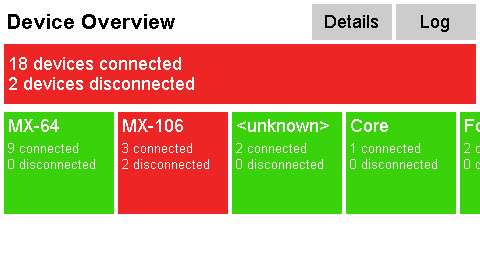
\includegraphics[scale=0.75]{img/device_overview.png}}
    \caption[Screenshot of the device overview]{
        Screenshot of the device overview. The top bar is red because at least one device (two in
        this case) is disconnected. The squares below the bar show the status of the devices of a
        specific model. They also turn red if at least one device is disconnected. The list containing
        them is horizontally scrollable. Each square can be clicked and will open the model overview
        for the corresponding model.
    }
\end{figure}

\clearpage
\paragraph{Model overview}

Displays the status and ID of each device of a certain model. Each device in the list can be clicked
to open the device details view and select that device. This view does not provide as much detail as
the device details view but it only shows devices of one particular model, making it easy to find
the exact device that is disconnected. The view is updated every \SI{500}{\milli\second}.

\begin{figure}[H]
    \centering
    \setlength{\fboxsep}{0mm}
    \fbox{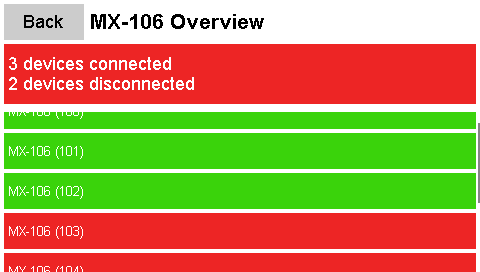
\includegraphics[scale=0.75]{img/model_overview.png}}
    \caption[Screenshot of the model overview]{
        Screenshot of the model overview. The top bar is red because at least one device for the
        selected model (MX-106) is disconnected. Below the bar is a scrollable list with an item for
        each device of the selected model. The device's ID is shown in parentheses and the item is
        colored red when it is disconnected. Clicking an item will navigate to the device details view
        and select the clicked device.
    }
\end{figure}

\clearpage
\paragraph{Device details view}

Displays all known values of single device's \textit{control table}. Different devices can be selected
by using the list on the left hand side. This view provides the maximum amount of detail per device
but makes it harder to determine the status of all connected devices at once. The view is updated every
\SI{500}{\milli\second}.

\begin{figure}[H]
    \centering
    \setlength{\fboxsep}{0mm}
    \fbox{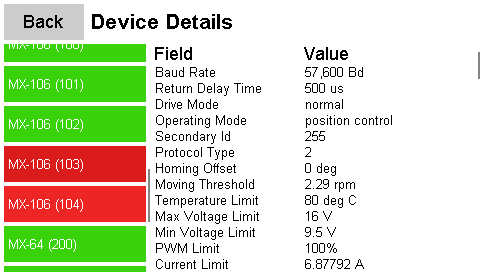
\includegraphics[scale=0.75]{img/device_details_view.png}}
    \caption[Screenshot of the device details view]{
        Screenshot of the device details view. The list on the left hand side contains an item for
        each connected device that is colored green when the device is connected and red otherwise.
        Clicking an item will select that device and show all values of its \textit{control table}
        in the table on the right hand side.
    }
\end{figure}

\clearpage
\paragraph{Log view}

Displays profiling information such as free memory and maximum and average processing times, as well
as the last 50 errors that occurred during packet processing. This view is mostly intended for debugging.
It has to be refreshed manually since a lot of errors may occur in short bursts, making it impossible
to actually read an individual error message.

\begin{figure}[H]
    \centering
    \setlength{\fboxsep}{0mm}
    \fbox{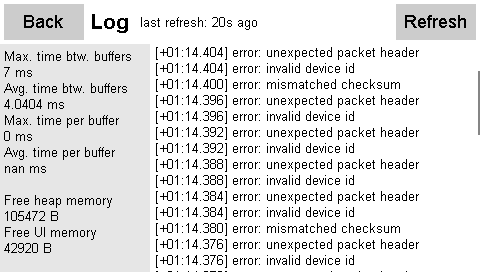
\includegraphics[scale=0.75]{img/log_view.png}}
    \caption[Screenshot of the log view]{
        Screenshot of the log view. The left hand side contains profiling information like processing
        times and free memory, the right hand side shows the 50 most recent error messages. The
        timestamps in the error log are relative to the start of the application. The view is only
        refreshed when the \textit{Refresh} button is clicked.
    }
\end{figure}

All of the views have to regularly access data shared with the packet processing task. While they
are holding the lock for this data, the packet processing task may be blocked on this lock. This
makes it extremely important to minimize the time spent holding any locks. All of the views do this
by copying the needed data before processing it. Thus, they only ever hold a lock to make copies,
which is relatively quick compared to updating the entire UI at the same time. This does decrease
the theoretical performance of the UI; however, the UI only needs to be fast enough to not appear
slow to the user. In comparison, the packet processing task has strict deadlines. If it is blocked
for too long, it will miss incoming data.

\subsection{Packet Processing Task}
\label{implementation/software/packet-processing-task}

The packet processing task is responsible for processing the data the UART connected to the \textit{RS-485}
bus receives. Since the bus has a data rate of \SI{2}{\mega{Bd}}, performance is crucial. Data must be
processed faster than it arrives in order to not lose any of it. At the same time, there needs to be
enough processing time left to also update to UI.

The code is designed to work with more than one bus at the same time. Each bus is associated with
a \lstinline{Connection} object. It holds the state of the packet parser, some profiling information
and a pointer to a buffer that stores received data. At the moment, only a single bus connected to
\textit{UART6} is supported.

\begin{lstlisting}[language=C++, caption={Main loop of the packet processing task}]
while (true) {
    for (auto& connection : connections) {
        if (connection.last_processing_start == 0) {
            connection.last_processing_start = HAL_GetTick();
        }

        process_buffer(log, connection, control_table_map);
    }

    vTaskDelay(4 / portTICK_PERIOD_MS);
}
\end{lstlisting}

The buffer is automatically filled by the DMA controller. It transfers the bytes from the UARTs
receive register and raises interrupts when half or the entire buffer has been filled. Once it has
been filled, the DMA controller starts at the beginning of the buffer again. The interrupt handler
sets a flag that determines which part of the buffer is now ready. As long as the data is processed
faster than it is received, no data will be lost. Even when the data is not processed quickly enough,
there will be no serious malfunctions. Some data may be corrupted but this will usually be detected
by the CRC checksums that are part of the ROBOTIS Dynamixel protocol (see section \ref{basics/dynamixel-protocol}).

The size of the buffer has a significant impact on the maximum time allowed before data is lost. A
larger buffer increases this time but also increases the latency. The latency can largely be ignored
because it is still low (for human time scales) given the possible buffer sizes. Latency would
increase drastically if there were no or only very little traffic on the bus, as data is only ever
processed once one half of the buffer is ready. Other than by memory contraints, the size of the buffer
is limited to \SI{65535}{B} by the size of the DMA controller's NDT register~\cite{mcu-ref-manual}.

The buffer's size is \SI{8192}{B}. This means that even assuming the absolute worst case, the maximum
amount of time for processing one half of the buffer is
$\frac{\SI{4096}{B}}{\SI{2}{\mega{Bd}} \mathbin{/} 8} \approx \SI{16}{\milli\second}$. Realistically,
the maximum amount of time will be higher for multiple reasons:

\begin{itemize}
    \item The baud rate of the bus is not equivalent to the bit rate of the incoming data, since
          this equation ignores overhead like stop bits.
    \item In practice it is impossible to have \SI{100}{\percent} load on the bus.
    \item The equation assumes that processing starts right after an interrupt signals that one half
          of the buffer is ready, and does not actually process a single byte. Normally, data is
          then being processed, which continuously moves the point at which a collision with the DMA
          controller can occur.
\end{itemize}

For these reasons, if the maximum amount of time between processing one half of the buffer never
exceeds \SI{16}{\milli\second}, there will be no data loss or corruption.

\begin{figure}[h]
    \centering
    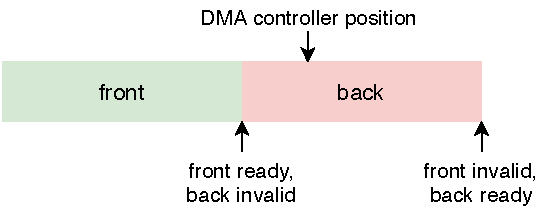
\includegraphics[scale=1.0]{img/dma_buffer.pdf}
    \caption[Layout of the DMA buffer]{
        After more than half of the DMA buffer has been filled, the front of it is ready and can be
        read. At the same time, the back of it is now invalid because the DMA controller is writing
        to it. The situation is reversed when the DMA controller has finished writing to the back
        and starts at the front again.
    }
\end{figure}

Since the buffer is written to by the DMA controller and then read by the CPU, the CPU must not cache
reads. This is accomplished by placing the buffer in the DTCM RAM section of the microcontroller's
memory. DTCM RAM is never cached~\cite{mcu-ref-manual}.

After processing one half of each buffer per bus, control is yielded to the UI task for \SI{4}{\milli\second}.
The UI can only be updated during this time. Increasing this time also increases the responsiveness
of the UI while increasing the time spent between the processing of data.

The \lstinline{process_buffer} function then parses packets until all the data in the ready buffer
has been consumed. Each successfully parsed packet is passed to \lstinline{ControlTableMap::receive},
which processes the contents of the packets. Errors and profiling information are passed to the
\lstinline{Log} object afterwards.

Due to this, the mutexes for the \lstinline{ControlTableMap} and the \lstinline{Log} object are
never locked at the same time. The UI task also never locks more than one of these mutexes at a time.
Holding only one lock at the same time prevents deadlocks.

The lock for the \lstinline{ControlTableMap} object is intentionally is held for almost the whole
duration of the call. Unlike with the UI task where holding the lock for a long time would block
the packet processing task, there is no task to block since the only other task is the UI task which
can only run when the packet processing explicitly yields control. Maximizing the time holding a
mutex removes the overhead of locking it multiple times.

\paragraph{Parser}

The \lstinline{Parser} is responsible for parsing packets from the ready part of a buffer. It
consumes bytes from a \mbox{\lstinline{Cursor}.} A \lstinline{Cursor} is essentially a pointer to
a part of the buffer that also tracks how many bytes have already been read. This enables a simple
API for the \lstinline{Parser} itself. Each call to the \lstinline{parse} method either parses one
packet successfully, encounters an error or parses a packet partially. In all cases, the \lstinline{Cursor}
tracks the current position and indicates when all bytes have been consumed, while the \lstinline{Parser}
holds state that must be retained across parses.

Most importantly, it stores the previous three bytes. When inspecting the next byte there are three
possible scenarios:

\begin{itemize}
    \item the byte and the previous three bytes are the header of a new packet
    \item the byte is stuffing (it can be ignored)
    \item the byte is a regular byte
\end{itemize}

In case the header of a packet is detected while already parsing a packet, an error is returned.
Returning early when encountering an error or only partially parsing a packet is possible because
the \lstinline{Parser} stores the part of the packet currently being parsed and the incremental
CRC checksum.

\begin{lstlisting}[language=C++, caption={Definition of the \lstinline{Packet} struct}]
struct Packet {
    DeviceId device_id;
    Instruction instruction;
    Error error;
    std::vector<uint8_t> data;
};
\end{lstlisting}

The speed of the \lstinline{Parser} is critical to performance. To avoid allocating memory while
parsing, the \lstinline{parse} method takes a pointer to a \lstinline{Packet} struct as argument.
Since packets are processed sequentially, the same \lstinline{Packet} struct can be reused. Packets
themselves can have different lengths but when defining a maximum allowed packet length, the memory
for a \lstinline{Packet} of that length can be preallocated. Defining a maximum packet length also
makes sense in order to avoid running out of memory due to packets with incorrect \textit{Length}
fields.

The \lstinline{Packet} struct represents both instruction and status packets since the only difference
between them is the addition of an \textit{Error} field for status packets (see section
\ref{basics/dynamixel-protocol}). For instruction packets the \lstinline{error} member can be ignored
because it will never contain an error.

\paragraph{ControlTableMap}

The \lstinline{ControlTableMap} object then processes these \lstinline{Packet} structs further.
Status packets are left as is but instruction packets are parsed into \lstinline{InstructionPacket}
structs. An \lstinline{InstructionPacket} is a discriminated union of structs for each instruction.
Because the instruction specific fields are part of the payload of a packet, parsing them is simple.
Unlike the packet parser, the instruction packet parser is just a function. It also reuses previous
\lstinline{InstructionPacket}s, but does allocate memory. Further optimization was not required to
achieve the desired performance.

\begin{lstlisting}[language=C++, caption={Definition of the \lstinline{InstructionPacket} struct}]
struct InstructionPacket {
    // constructors, destructor and member functions omitted

    Instruction instruction;
    union {
        PingArgs ping;
        ReadArgs read;
        WriteArgs write;
        RegWriteArgs reg_write;
        ActionArgs action;
        FactoryResetArgs factory_reset;
        RebootArgs reboot;
        ClearArgs clear;
        SyncReadArgs sync_read;
        SyncWriteArgs sync_write;
        BulkReadArgs bulk_read;
        BulkWriteArgs bulk_write;
    };
};
\end{lstlisting}

For every received instruction packet, the \lstinline{ControlTableMap} records the devices that are
expected to respond. When a new instruction packet is received, a counter for each device from which
a status packet was not received is incremented. These counters are reset when a status packet from
the corresponding device has been received. Devices that have not responded to more than four instruction
packets are considered disconnected.

\textit{Ping} instructions are handled differently: the status packet responding to a \textit{Ping}
instruction contains the model number of the device. The model number is used to register a new device.
Each device is mapped to a \lstinline{ControlTable} object that stores the current state of the device's
\textit{control table}. If the device is not registered, has a different or an unknown model number,
a new \lstinline{ControlTable} matching the model number is allocated. A device's model can be unknown
if status packets from that device have been received without previously receiving the response to a
\textit{Ping} instruction.

Whenever data is written to or read from a device, the written or read data is also updated for the
\lstinline{ControlTable} object belonging to that device. This is the data that is displayed by the
UI. Only the following instructions are handled properly:

\begin{itemize}
    \item \textit{Ping}
    \item \textit{Read}
    \item \textit{Write}
    \item \textit{Sync Read}
    \item \textit{Sync Write}
    \item \textit{Bulk Read}
    \item \textit{Bulk Write}
\end{itemize}

The remaining instructions are mostly ignored but still used for detecting disconnected devices.
Adding support for them would be a significant effort especially considering that these instructions
do not appear in most traffic. The current implementation also assumes that writes do not require a
status packet response, as this is how the \textit{Wolfgang} robot platform is configured.

The \lstinline{ControlTable} objects are identified by the ID of the device they belong to. Initially,
a \lstinline{std::unordered_map} was used but the performance proved to be insufficient. Instead, the
objects are stored in a custom data structure. It takes advantage of the fact that device IDs are
only one byte and that \lstinline{ControlTable} objects must be accessed through a pointer (four bytes
on a Cortex M7 processor~\cite{mcu-ref-manual}). The objects are simply stored in an array that is
indexed by the device ID. An additional boolean flag indicates presence or absence of the object. The
entire array only requires $256 \cdot (4 + 1 + 3) = \SI{2048}{B}$ of memory (this includes three bytes
of padding).
This solution trades memory and iteration speed for fast access times. Since objects must be accessed
for almost every received packet, this provides a serious speedup compared to \lstinline{std::unordered_map}.

\paragraph{ControlTable}

The \textit{control table} of each device is represented by a \lstinline{ControlTable} object. For
each device model there is a different sub class of \lstinline{ControlTable}. Most received packets
update the \lstinline{ControlTable} object of at least one device, performance is thus an important
design consideration. Adding or changing the \lstinline{ControlTable} of a device has to be easy.

The interface definition of the \lstinline{ControlTable} base class can be seen in listing
\ref{implementation/software/packet-processing-task/control-table-def}. \lstinline{is_unknown_model}
determines if the model number is known and \lstinline{model_number} returns its value if present.
\lstinline{set_firmware_version} is called when the firmware version is reported by the response
to a \textit{Ping} instruction. \lstinline{device_name} simply returns a human readable name of the
model represented by the \lstinline{ControlTable}. It is used for display purposes only.

\begin{lstlisting}[
    language=C++,
    caption={Definition of the \lstinline{ControlTable} class},
    label=implementation/software/packet-processing-task/control-table-def,
]
class ControlTable {
  public:
    virtual ~ControlTable() = default;

    virtual std::unique_ptr<ControlTable> clone() const = 0;

    virtual bool is_unknown_model() const;

    virtual uint16_t model_number() const = 0;

    virtual void set_firmware_version(uint8_t version) = 0;

    virtual const char* device_name() const = 0;

    virtual ControlTableMemory& memory() = 0;

    virtual const ControlTableMemory& memory() const = 0;

    virtual const std::vector<ControlTableField>& fields() const = 0;

    bool write(uint16_t start_addr, const uint8_t* buf, uint16_t len);

    std::vector<std::pair<const char*, std::string>> fmt_fields() const;
};
\end{lstlisting}

The core functionality of \lstinline{ControlTable} class uses the \lstinline{memory} and
\lstinline{fields} methods. The \lstinline{ControlTableMemory} object returned by a call to
\lstinline{memory} is responsible for storing the actual data. It is made up of multiple
\lstinline{Segment}s that each describe a region of memory:

\begin{itemize}
    \item data segments are some memory starting at a certain address
    \item indirect address segments allow redirecting addresses (required to support ROBOTIS
          \textit{MX-64} and \textit{MX-106} servos)
    \item unknown segments allow no reads and ignore writes (these are used when the model number
          is not known)
\end{itemize}

The descriptions are used by the \lstinline{ControlTableMemory} object to map data contained in
packets to a single, flat byte array. Calls to the \lstinline{write} method of a \lstinline{ControlTable}
object are forwarded to the \lstinline{ControlTableMemory}. By using an accessor, only one virtual
call has to be performed, even when writing more than one byte.

The \lstinline{fields} method returns a description of all fields in a device's \textit{control table}.
Each \lstinline{ControlTableField} stores the address, type, name, and default value of a single
field. It also contains a function for formatting the value of the field as a human readable string.

\begin{lstlisting}[language=C++, caption={Definition of the control table fields of a Rhoban DXL Board}]
const std::vector<ControlTableField> CoreBoardControlTable::FIELDS{
  ControlTableField::new_uint16(0, "Model Number", CoreBoardControlTable::MODEL_NUMBER, fmt_number),
  ControlTableField::new_uint8(2, "Firmware Version", 0, fmt_number),

  ControlTableField::new_uint16(10, "LED", 0, fmt_bool_on_off),
  ControlTableField::new_uint16(12, "Power", 0, fmt_number),
  ControlTableField::new_uint32(14, "RGB LED 1", 0, fmt_core_rgb),
  ControlTableField::new_uint32(18, "RGB LED 2", 0, fmt_core_rgb),
  ControlTableField::new_uint32(22, "RGB LED 3", 0, fmt_core_rgb),
  ControlTableField::new_uint16(26, "VBAT", 0, fmt_core_voltage),
  ControlTableField::new_uint16(28, "VEXT", 0, fmt_core_voltage),
  ControlTableField::new_uint16(30, "VCC", 0, fmt_core_voltage),
  ControlTableField::new_uint16(32, "VDXL", 0, fmt_core_voltage),
  ControlTableField::new_uint16(34, "Current", 0, fmt_core_current),
  ControlTableField::new_uint16(36, "Power On", 0, fmt_core_power_on),
};
\end{lstlisting}

These descriptions are used by the \lstinline{fmt_fields} method. It reads the current value of a
field from the \lstinline{ControlTableMemory} and formats it using the formatting function. This
function is used to display the contents of a device's \textit{control table}. Formatting all fields
is quite slow, which is why the UI task first copies the entire \lstinline{ControlTable} object using
the \lstinline{clone} method. It effectively acts as a virtual copy constructor.

To add support for a new device model, one only has to create a new sub class of \lstinline{ControlTable}
and construct an instance of it when a response to a \textit{Ping} instruction is received. Currently,
the following device models are supported:

\begin{itemize}
    \item ROBOTIS MX-64 servos (\url{http://emanual.robotis.com/docs/en/dxl/mx/mx-64-2/})
    \item ROBOTIS MX-106 servos (\url{http://emanual.robotis.com/docs/en/dxl/mx/mx-106-2/})
    \item Rhoban DXL Boards (\url{https://github.com/Rhoban/DXLBoard})
    \item BitFoot foot pressure sensors (\url{https://github.com/bit-bots/bit_foot})
    \item \textit{Hamburg Bit-Bots} IMU modules (\url{https://github.com/bit-bots/imu_module})
\end{itemize}

\chapter{Evaluation}
\label{evaluation}

% TODO: consistently use `experiment` where appropriate

This chapter evaluates the performance of the implementation described in chapter \ref{implementation}.
Two measurements were taken to assess the performance:

\begin{itemize}
    \item The time required to process the ready half of the receive buffer (see subsection
          \ref{implementation/software/packet-processing-task}). This measurement will be called
          \textbf{time per buffer} in the following.
    \item The time that passes between two calls of \lstinline{process_buffer} function (again, see
          subsection \ref{implementation/software/packet-processing-task}). This measurement will be
          called \textbf{time between buffers} in the following.
\end{itemize}

The \textit{time per buffer} measures the performance of the part of the system that actually deals
with incoming data. It does not measure idle time and synchronization overhead. The
\textit{time between buffers} on the other hand measures the performance of the entire system. It
indicates how much time passes between two opportunities to process incoming data. This means that
if this time does not exceed the maximum amount of time of \SI{16}{\milli\second} calculated in
subsection \ref{implementation/software/packet-processing-task}, no incoming data will be lost.

In addition, the perceived responsiveness of the UI is also reported. These observations are entirely
subjective and only meant to give an impression of the responsiveness to be expected.

% TODO: actually tag the branch tip
The source code of the firmware and scripts used for measurements as well as the results can be found
at \url{https://github.com/Laegluin/embedded_debug_interface_for_robots/tree/thesis-benchmark-ref}.
The version used for measurements is tagged as \lstinline{thesis-benchmark-ref}.

All code was compiled with GCC 6.3.1 with maximum optimizations, link-time optimization and no
exception support (\lstinline{-O3 -flto -fno-exceptions}).

Section \ref{evaluation/measurement-method} describes the method used to obtain the measurements and
section \ref{evaluation/results} presents the results.

\section{Measurement Method}
\label{evaluation/measurement-method}

The FT232R USB to UART converter listed in section \ref{implementation/hardware} was used to simulate
an actual \textit{RS-485} bus. Three different kinds of simulated traffic were used:

\begin{itemize}
    \item A trace of real traffic from the bus of a robot of the \textit{Hamburg Bit-Bots}.
    \item Synthetic traffic of 20 devices consisting of \textit{Ping} instructions followed by
          \textit{Read}, \textit{Write}, \textit{Sync Read}, \textit{Sync Write}, \textit{Bulk Read}
          and \textit{Bulk Write} instructions for each device, repeated 300 times.
    \item Synthetic traffic of 20 devices that are constantly responding to \textit{Ping} instructions.
          Devices change their model number after each \textit{Ping} instruction.
\end{itemize}

The simulated traffic was sent to the USB to UART converter in two ways:

\begin{itemize}
    \item the entire file of simulated traffic at once
    \item one packet at a time, with \SI{100}{\micro\second} delay per packet
\end{itemize}

A python script was used to send the simulated traffic. Output buffering was disabled. To minimize
the system call overhead when not adding any delay, the files containing the simulated traffic all
had a size of at least \SI{400}{KiB}. When the file was smaller, it was made bigger by simply
repeating the contents.

All combinations of the aforementioned parameters (for a total of six different combinations) were
used for measurements. Before starting the measurements, the microcontroller was reset and every
view of the UI was opened at least once to ensure that every view would be updated. Measurements
were taken for at least \SI{80}{\second} after reset.

The firmware had to be modified slightly to allow for collection of the measurements. An additional
timer was used to generate an interrupt every \SI{0.1}{\milli\second}. The interrupt handler incremented
a counter every time it was called. This counter was used in calls to \lstinline{process_buffer} to
determine the current time. Thus, every measurement has an accuracy of \SI{0.1}{\milli\second}.

Measurements were stored on external RAM. After enough measurements had been taken, the microcontroller
was halted using the debugger. The debugger was then used to dump the memory that stored the
measurements. The raw data was converted to a JSON file and then plotted using two python scripts.

The interrupts generated by the additional timer and the extra code to store the measurements on
comparatively slow external RAM imposed overhead that is not present during normal execution. As a
consequence, all times measured are an upper bound on the expected values. The differences should be
minimal, however.

\section{Results}
\label{evaluation/results}

This section presents the results of the measurements for each of the six combinations mentioned
above. Every combination is presented in a separate subsection. There are four different plots
for each combination. The scatter plots show the \textit{time per buffer} and
\textit{time between buffers} over time. Since each data point represents a duration, points in the
plots are placed at the geometric mean of the start and end point of the duration. The histograms
show the distribution of durations for each scatter plot.

The first \SI{20}{\second} of measurements were discarded to allow for the manual setup, the next
\SI{60}{\second} were used to generate the following plots.


\subsection{Trace, no delay}
\label{evaluation/results/trace-no-delay}

\begin{figure}[H]
    \centering

    \begin{subfigure}[t]{0.5\textwidth}
        \centering
        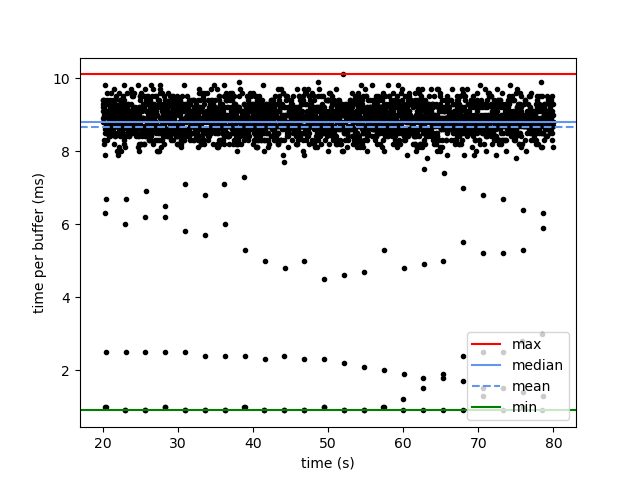
\includegraphics[scale=0.45]{img/trace_no_wait_per_buffer_scatter.png}
        \caption{Scatter plot of \textit{time per buffer}}
    \end{subfigure}%
    \begin{subfigure}[t]{0.5\textwidth}
        \centering
        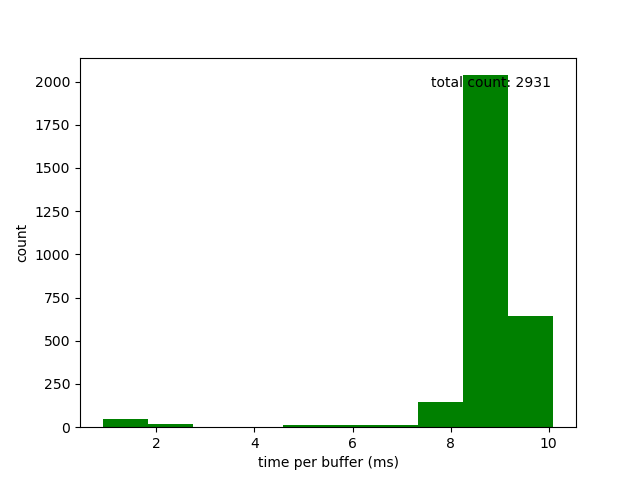
\includegraphics[scale=0.45]{img/trace_no_wait_per_buffer_hist.png}
        \caption{Histogram of \textit{time per buffer}}
    \end{subfigure}

    \begin{subfigure}[t]{0.5\textwidth}
        \centering
        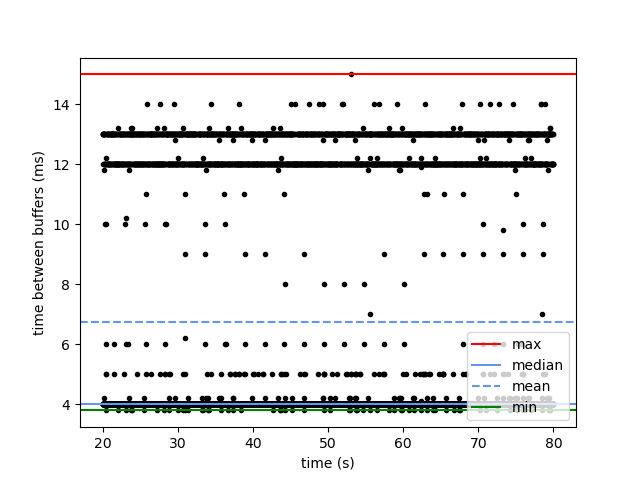
\includegraphics[scale=0.45]{img/trace_no_wait_between_buffers_scatter.png}
        \caption{Scatter plot of \textit{time between buffers}}
    \end{subfigure}%
    \begin{subfigure}[t]{0.5\textwidth}
        \centering
        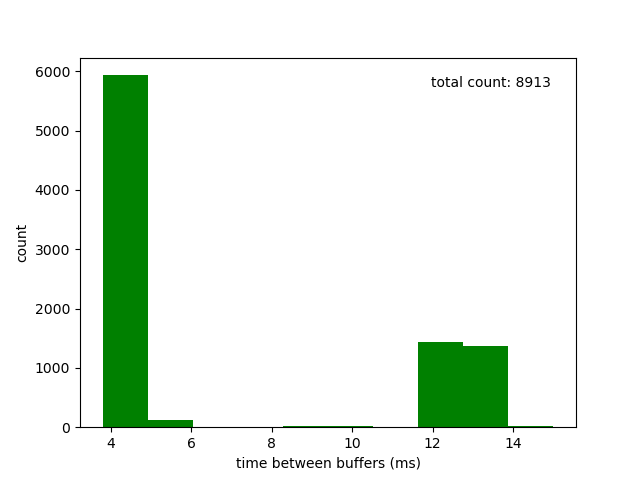
\includegraphics[scale=0.45]{img/trace_no_wait_between_buffers_hist.png}
        \caption{Histogram of \textit{time between buffers}}
    \end{subfigure}

    \caption{\textit{Time per buffer} and \textit{time between buffers} for trace traffic with no delay}
    \label{evaluation/results/trace-no-delay/plots}
\end{figure}

\paragraph{UI responsiveness}

The UI was responsive, there was regular but short stuttering.
\bigbreak

Most of the measurements of \textit{time per buffer} are clustered around \SIrange{8}{10}{\milli\second}.
There are noticeable exceptions that occur at regular intervals. These are most likely packets that
were not transmitted correctly at the time the trace was recorded. Because they were malformed, they
were ignored after parsing, leading to less time spent processing the buffer that contained these
errors. Transmission errors that occurred during the measurements are unlikely to have had a significant
impact due to the extremely short cable length. In addition, these errors would not appear at regular
intervals, while recorded errors would be repeated every time the trace is repeated, which happened
frequently since the size of the trace was only \SI{516}{KiB}.

There are two distincts spikes in the \textit{time between buffers}. The higher spike is caused by
those measurements that were taken while a buffer was being processed. Most of the measurements a
around \SI{4}{\milli\second}. These are the measurements taken when there was no data to process.
They are the majority, indicating that higher data rates could be handled without a problem.

It is unclear why the \textit{time between buffers} is so tightly clustered around certain times.
It is possible that these clusters were caused by synchronization with one of the mutexes. Since the
time the UI task was holding a lock was always the same and since FreeRTOS could only preempt a task
every millisecond, there was only a very limited set of possible wait times for the packet processing
task. These wait times may have been what caused the tight clustering.

\subsection{Trace, \SI{100}{\micro\second} delay}
\label{evaluation/results/trace-100us-delay}

\begin{figure}[H]
    \centering

    \begin{subfigure}[t]{0.5\textwidth}
        \centering
        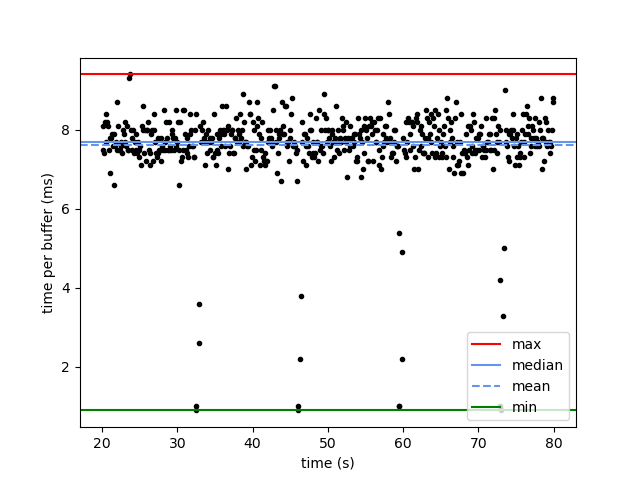
\includegraphics[scale=0.45]{img/trace_wait_100us_per_buffer_scatter.png}
        \caption{Scatter plot of \textit{time per buffer}}
    \end{subfigure}%
    \begin{subfigure}[t]{0.5\textwidth}
        \centering
        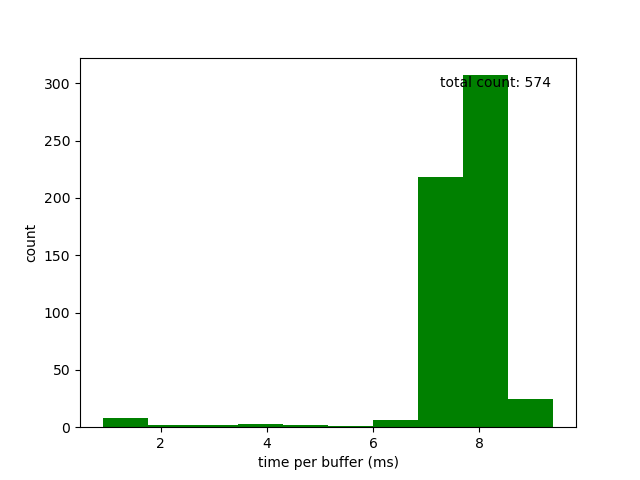
\includegraphics[scale=0.45]{img/trace_wait_100us_per_buffer_hist.png}
        \caption{Histogram of \textit{time per buffer}}
    \end{subfigure}

    \begin{subfigure}[t]{0.5\textwidth}
        \centering
        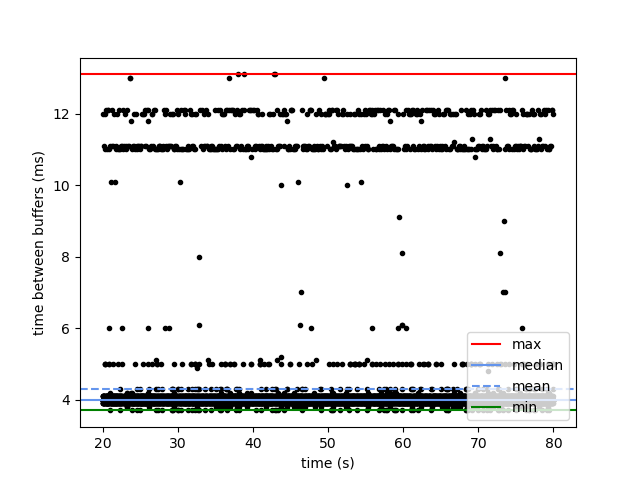
\includegraphics[scale=0.45]{img/trace_wait_100us_between_buffers_scatter.png}
        \caption{Scatter plot of \textit{time between buffers}}
    \end{subfigure}%
    \begin{subfigure}[t]{0.5\textwidth}
        \centering
        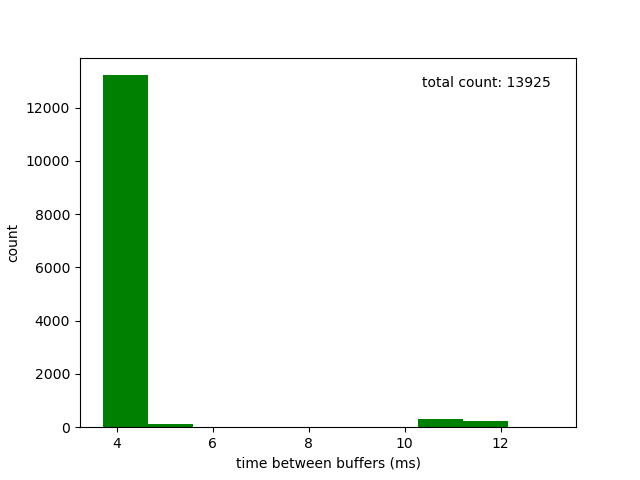
\includegraphics[scale=0.45]{img/trace_wait_100us_between_buffers_hist.png}
        \caption{Histogram of \textit{time between buffers}}
    \end{subfigure}

    \caption{\textit{Time per buffer} and \textit{time between buffers} for trace traffic with \SI{100}{\micro\second} delay}
    \label{evaluation/results/trace-100us-delay/plots}
\end{figure}

\paragraph{UI responsiveness}

The UI was responsive, there was only occasional minimal stuttering.
\bigbreak

All measurements look extremely similar to those with no delay. Since the additional delay reduced
the effective data rate, there were less packets processed in the same time frame and the influence
of malformed packets was not as severe.

The \textit{time between buffers} is absolutely dominated by measurements taken when there was no
data to process. This is not suprising, as even less time was spent processing data when there was
also a delay per packet.

\subsection{Synthetic Read/Write instructions, no delay}
\label{evaluation/results/synthetic-read-write-instructions-no-delay}

\begin{figure}[H]
    \centering

    \begin{subfigure}[t]{0.5\textwidth}
        \centering
        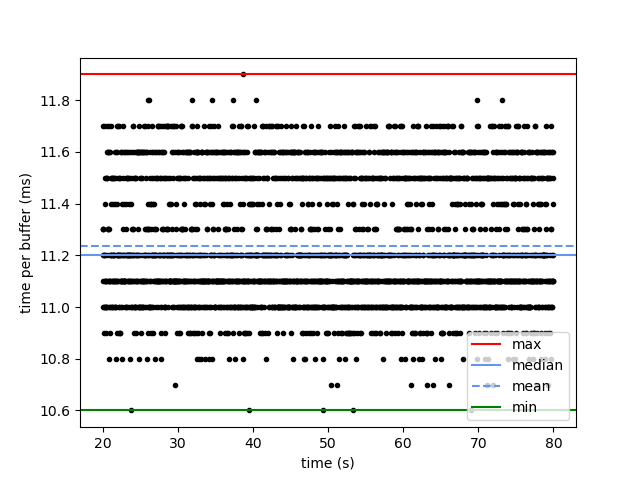
\includegraphics[scale=0.45]{img/synthetic_read_writes_no_wait_per_buffer_scatter.png}
        \caption{Scatter plot of \textit{time per buffer}}
    \end{subfigure}%
    \begin{subfigure}[t]{0.5\textwidth}
        \centering
        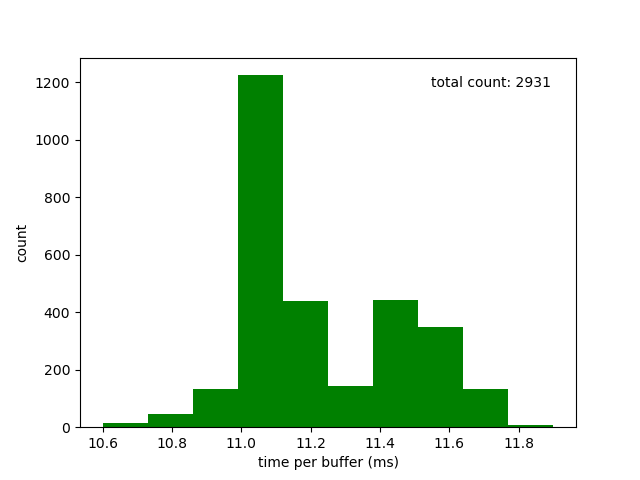
\includegraphics[scale=0.45]{img/synthetic_read_writes_no_wait_per_buffer_hist.png}
        \caption{Histogram of \textit{time per buffer}}
    \end{subfigure}

    \begin{subfigure}[t]{0.5\textwidth}
        \centering
        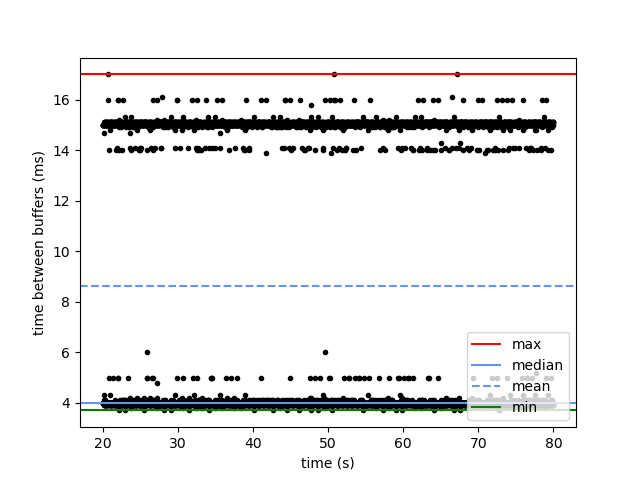
\includegraphics[scale=0.45]{img/synthetic_read_writes_no_wait_between_buffers_scatter.png}
        \caption{Scatter plot of \textit{time between buffers}}
    \end{subfigure}%
    \begin{subfigure}[t]{0.5\textwidth}
        \centering
        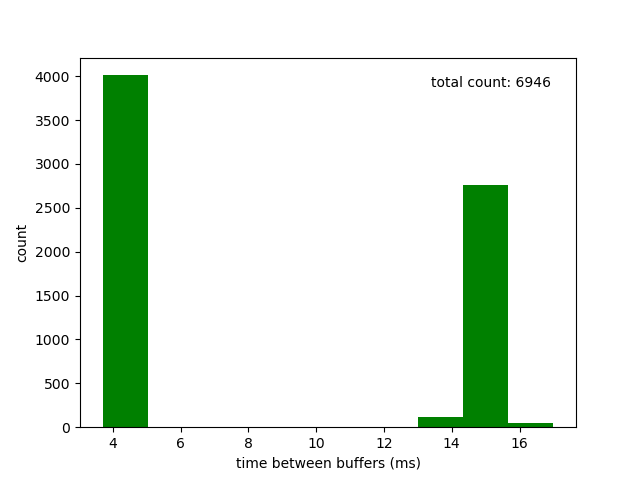
\includegraphics[scale=0.45]{img/synthetic_read_writes_no_wait_between_buffers_hist.png}
        \caption{Histogram of \textit{time between buffers}}
    \end{subfigure}

    \caption{\textit{Time per buffer} and \textit{time between buffers} for synthetic read/write traffic with no delay}
    \label{evaluation/results/synthetic-read-write-instructions-no-delay/plots}
\end{figure}

\paragraph{UI responsiveness}

The UI was still usable but there was heavy stuttering. Using the UI was not pleasant.
\bigbreak

Compared to the results with the recorded trace, there are almost no outliers in the measurements.
The synthetic nature of the data is clearly visible. Measurements are extremely clustered and all
clusters are very close to each other.

These clusters were most likely caused by the different types of packets that are part of the data.
The same types of packets were always sent as a sequence. Every type had a slightly different length
and took a slightly different path through the program. This did not make a significant difference to
the overall time but it was enough to consistently change the time it took to process a buffer,
depending on the types of packets it contained.

\subsection{Synthetic Read/Write instructions, \SI{100}{\micro\second} delay}
\label{evaluation/results/synthetic-read-write-instructions-100us-delay}

\begin{figure}[H]
    \centering

    \begin{subfigure}[t]{0.5\textwidth}
        \centering
        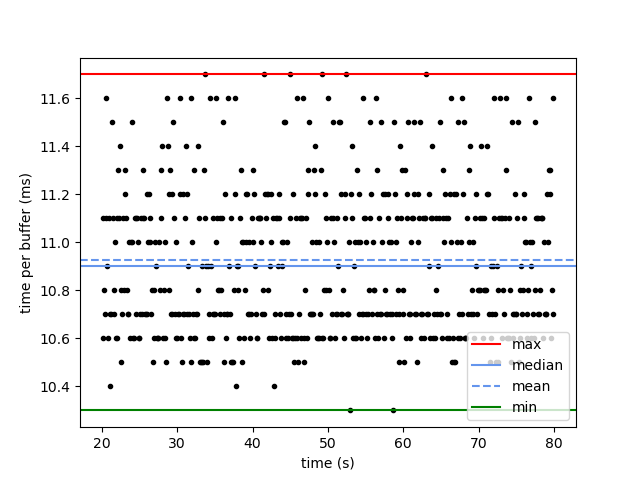
\includegraphics[scale=0.45]{img/synthetic_read_writes_wait_100us_per_buffer_scatter.png}
        \caption{Scatter plot of \textit{time per buffer}}
    \end{subfigure}%
    \begin{subfigure}[t]{0.5\textwidth}
        \centering
        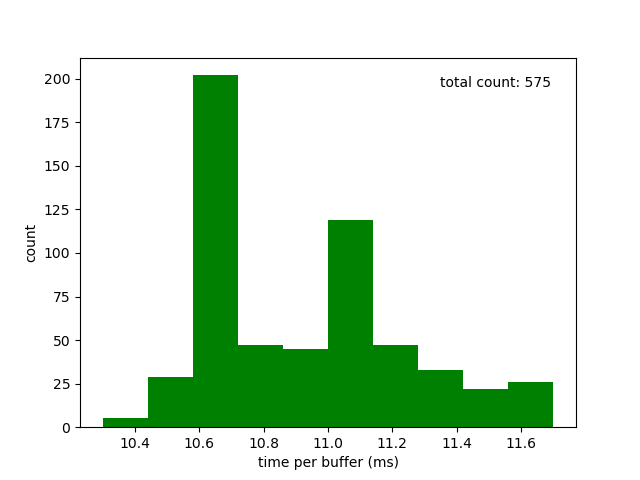
\includegraphics[scale=0.45]{img/synthetic_read_writes_wait_100us_per_buffer_hist.png}
        \caption{Histogram of \textit{time per buffer}}
    \end{subfigure}

    \begin{subfigure}[t]{0.5\textwidth}
        \centering
        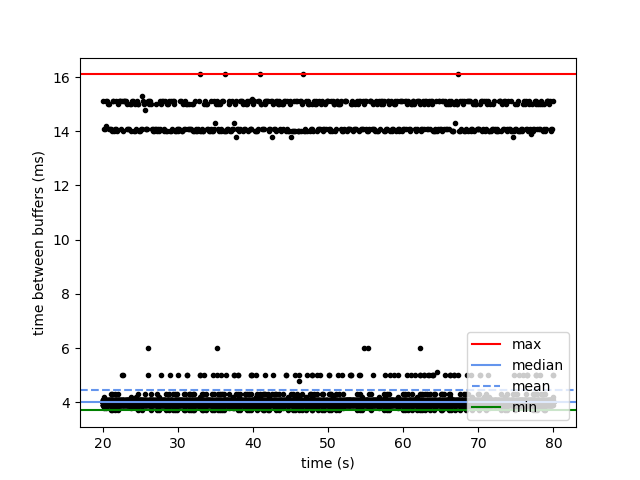
\includegraphics[scale=0.45]{img/synthetic_read_writes_wait_100us_between_buffers_scatter.png}
        \caption{Scatter plot of \textit{time between buffers}}
    \end{subfigure}%
    \begin{subfigure}[t]{0.5\textwidth}
        \centering
        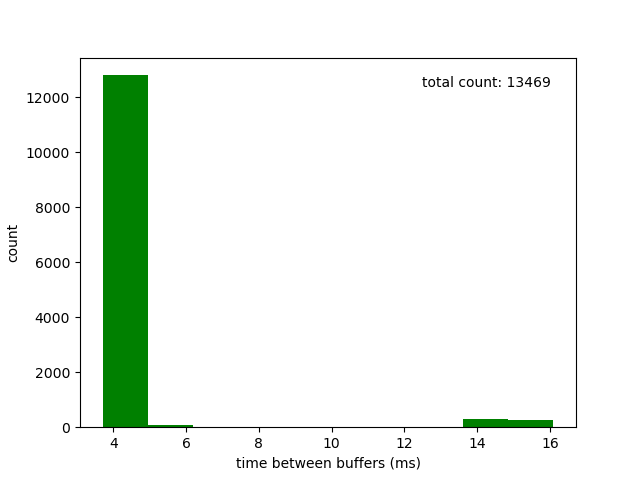
\includegraphics[scale=0.45]{img/synthetic_read_writes_wait_100us_between_buffers_hist.png}
        \caption{Histogram of \textit{time between buffers}}
    \end{subfigure}

    \caption{\textit{Time per buffer} and \textit{time between buffers} for synthetic read/write traffic with \SI{100}{\micro\second} delay}
    \label{evaluation/results/synthetic-read-write-instructions-100us-delay/plots}
\end{figure}

\paragraph{UI responsiveness}

The UI was responsive, there was only occasional short stuttering.
\bigbreak

Like the results with the recorded trace, results when adding a delay per packet are very similar to
those without delay. Again, clusters in the \textit{time per buffer} plots are less pronounced as
there are less measurements and the measurements for the \textit{time between buffers} are dominated
by constant overhead.

\subsection{Synthetic Ping instructions, no delay}
\label{evaluation/results/synthetic-ping-instructions-no-delay}

\begin{figure}[H]
    \centering

    \begin{subfigure}[t]{0.5\textwidth}
        \centering
        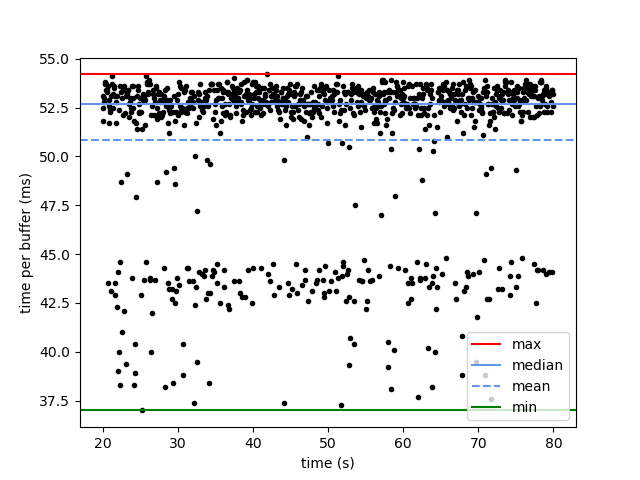
\includegraphics[scale=0.45]{img/synthetic_pings_no_wait_per_buffer_scatter.png}
        \caption{Scatter plot of \textit{time per buffer}}
    \end{subfigure}%
    \begin{subfigure}[t]{0.5\textwidth}
        \centering
        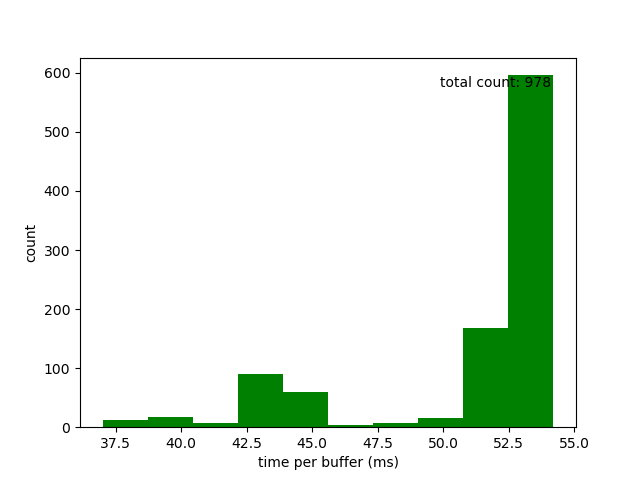
\includegraphics[scale=0.45]{img/synthetic_pings_no_wait_per_buffer_hist.png}
        \caption{Histogram of \textit{time per buffer}}
    \end{subfigure}

    \begin{subfigure}[t]{0.5\textwidth}
        \centering
        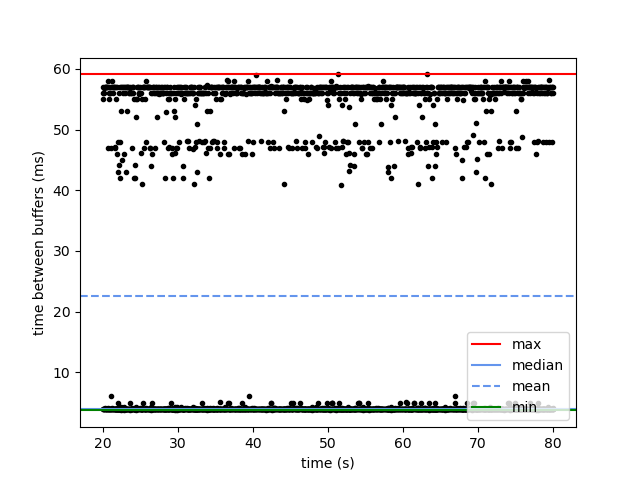
\includegraphics[scale=0.45]{img/synthetic_pings_no_wait_between_buffers_scatter.png}
        \caption{Scatter plot of \textit{time between buffers}}
    \end{subfigure}%
    \begin{subfigure}[t]{0.5\textwidth}
        \centering
        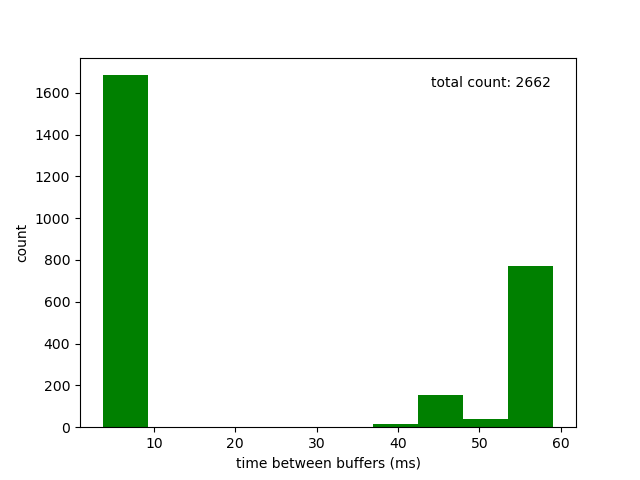
\includegraphics[scale=0.45]{img/synthetic_pings_no_wait_between_buffers_hist.png}
        \caption{Histogram of \textit{time between buffers}}
    \end{subfigure}

    \caption{\textit{Time per buffer} and \textit{time between buffers} for synthetic ping traffic with no delay}
    \label{evaluation/results/synthetic-ping-instructions-no-delay/plots}
\end{figure}

\paragraph{UI responsiveness}

The UI was not responsive at all. While it was still possible to use, scrolling did not work properly
and any action caused significant and noticeable delays.
\bigbreak

The results for the \textit{time per buffer} are significantly worse than any other results. The
maximum \textit{time per buffer} exceeds \SI{50}{\milli\second}. There are also many outliers. These
outliers were most likely caused by errors during parsing: since the buffers were not processed
quickly enough, the DMA controller was overwriting buffers as they were being read.

The \textit{time between buffers} reflects the measurements for \textit{time per buffer}. However,
it is notable that there are many measurements of only about \SI{4}{\milli\second}, even though the
processing was too slow. This is because after processing one buffer, there was a high likelyhood
that the next buffer was not currently ready. Data was not lost during these waits but during
processing itself, meaning that the amount of waits only decreased because more time was spent
processing data.

Because so much time was spent processing data, the amount of time dedicated to the UI decreased and
the latency increased. The high latencies caused problems with input handling since it could not be
processed in time. Less time for the UI task also meant the real time required for rendering the UI
increased.

\subsection{Synthetic Ping instructions, \SI{100}{\micro\second} delay}
\label{evaluation/results/synthetic-ping-instructions-100us-delay}

\begin{figure}[H]
    \centering

    \begin{subfigure}[t]{0.5\textwidth}
        \centering
        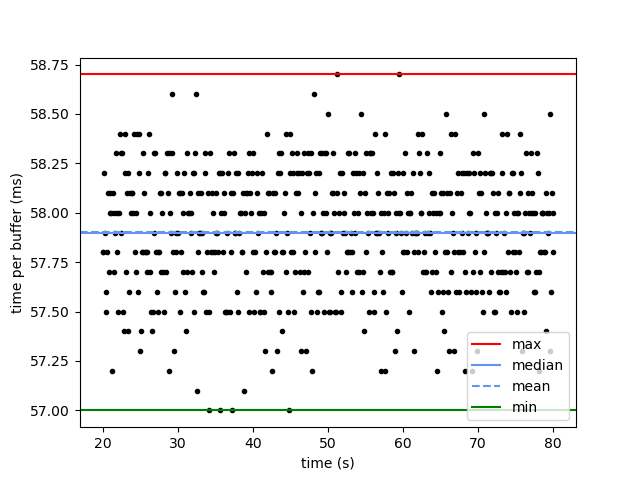
\includegraphics[scale=0.45]{img/synthetic_pings_wait_100us_per_buffer_scatter.png}
        \caption{Scatter plot of \textit{time per buffer}}
    \end{subfigure}%
    \begin{subfigure}[t]{0.5\textwidth}
        \centering
        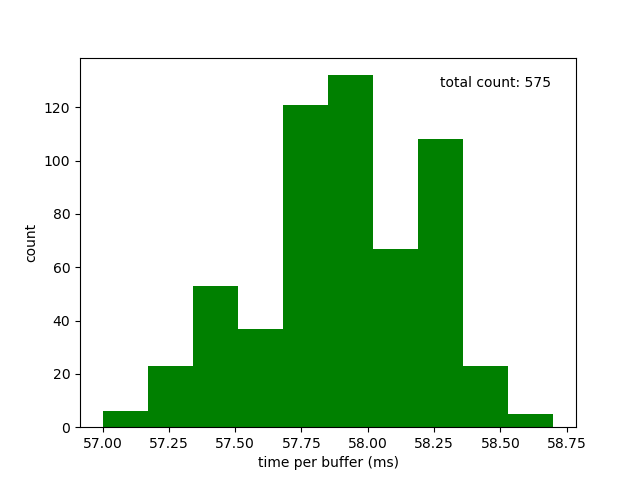
\includegraphics[scale=0.45]{img/synthetic_pings_wait_100us_per_buffer_hist.png}
        \caption{Histogram of \textit{time per buffer}}
    \end{subfigure}

    \begin{subfigure}[t]{0.5\textwidth}
        \centering
        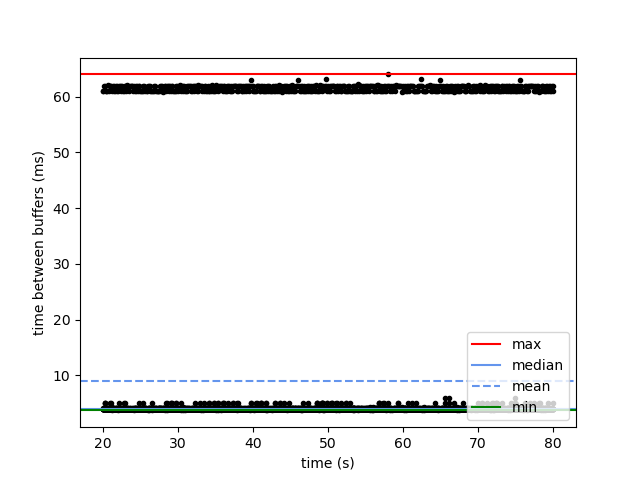
\includegraphics[scale=0.45]{img/synthetic_pings_wait_100us_between_buffers_scatter.png}
        \caption{Scatter plot of \textit{time between buffers}}
    \end{subfigure}%
    \begin{subfigure}[t]{0.5\textwidth}
        \centering
        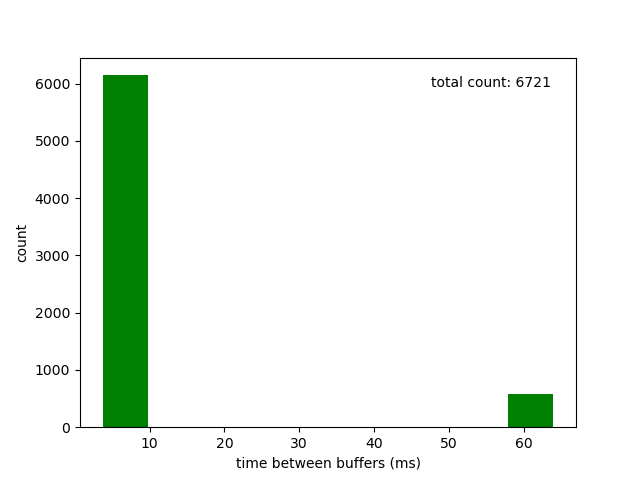
\includegraphics[scale=0.45]{img/synthetic_pings_wait_100us_between_buffers_hist.png}
        \caption{Histogram of \textit{time between buffers}}
    \end{subfigure}

    \caption{\textit{Time per buffer} and \textit{time between buffers} for synthetic ping traffic with \SI{100}{\micro\second} delay}
    \label{evaluation/results/synthetic-ping-instructions-100us-delay/plots}
\end{figure}

\paragraph{UI responsiveness}

The UI was mostly usable but there was significant stuttering. Scrolling mostly worked but was not
pleasant to use. The were noticeable but not significant delays when interacting with buttons. 
\bigbreak

Results with delay per packet look remarkably similar to those with synthetic \textit{Read} and
\textit{Write} instructions. The only difference is that all times increased drastically to about
\SIrange{57}{59}{\milli\second}. The reason is that while the average \textit{time per buffer} was
still about four times higher than the allowed maximum of \SI{16}{\milli\second}, the delay per
packet slowed down the effective data rate enough to make the actual allowed maximum greater than
the measured maximum \textit{time per buffer}.

This is also the reason the UI was so much more responsive than without any delay. The problems
caused by high latencies were still present but the UI task did have enough time to render the UI
at a sufficient speed.

\chapter{Discussion}
\label{discussion}

This chapter discusses the results gathered from the experiments that were presented and evaluated in
chapter \ref{evaluation}.
\bigbreak

All of the experiments except for \ref{evaluation/results/synthetic-ping-instructions-no-delay} and
\ref{evaluation/results/synthetic-ping-instructions-100us-delay} showed a maximum \textit{time between buffers}
of below or slightly above \SI{16}{\milli\second}. This means that in practice, the implementation is
performant enough to not lose any data, especially considering that a bus load of \SI{100}{\percent}
is not possible in reality.

It is clear that there is a constant overhead of about \SI{4}{\milli\second} in the
\textit{time between buffers}. This overhead can be seen as the median \textit{time between buffers}
in all experiments. This overhead is not small; compared to the approximate maximum of \SI{16}{\milli\second},
it is \SI{25}{\percent} of the entire time spent.

From both experiments that used synthetic \textit{Ping} instructions as data it is apparent that
\textit{Ping} instructions are the absolute worst case when it comes to processing time. This is
not surprising considering that \textit{Ping} instructions may require allocating a new
\lstinline{ControlTable} object. However, these allocations are only necessary when the model number
changes constantly as was the case in these two experiments. This is simply not a realistic scenario;
in practice, \textit{Ping} instructions are incredible rare, usually only sent when the master
connects to the bus for the first time.

The number of \textit{Ping} instructions in the other experiments was already higher than to be expected
because the data they used contained at least one \textit{Ping} instruction and response for every device.
This means that \textit{Ping} instructions were sent every time the data was repeated. This unusually
high frequency did not impact performance in any meaningful way, however. All four experiments processed
the incoming data in time.

Generally, the amount of load on the bus was noticeable when interacting with the UI. It manifested
as periodic increases in latency and low framerate. These became especially severe when the load was
too high to be processed in time.

This is a direct consequence of how the UI and the data processing task are configured. Since the UI
task is only assigned a fixed amount of time after all incoming data in one half of the buffer has
been processed, higher processing times decrease the overall amount time spent updating the UI.

While this only seriously affected the UI once incoming data was already getting lost, the user
experience was still not acceptable. There is certainly room for improvement, either by optimizing
the firmware, redesigning the way the priorities of the two tasks are handled or by switching to
hardware with greater processing power.

\chapter{Conclusion and Future Work}
\label{conclusion-and-future-work}

This chapter gives a conclusion on the work done as well as the results presented in section
\ref{conclusion-and-future-work/conclusion}. Section \ref{conclusion-and-future-work/future-work}
discusses possible future work.

\section{Conclusion}
\label{conclusion-and-future-work/conclusion}

In this thesis firmware for the STM32F7508-DK board has been developed that allows monitoring and
debugging the status of devices connected to a ROBOTIS Dynamixel Protocol 2.0 based bus. The targeted
\textit{Wolfgang} robot platform uses \textit{RS-485} but any bus compatible with a UART interface
can be used. Like with \textit{RS-485}, a transceiver or converter has to be used to interface the
bus with the board itself. It is also possible to directly connect a bus using TTL logic levels
(\SIrange{3.3}{5}{\volt}). This is effectively what was done during testing and evaluation.

The STM32F7508-DK board is well suited for the development of graphical applications. Because the
touchscreen display is already part of the board, no further assembly was required. The speed of
the STM32F750N8H6 microcontroller is sufficient but any less powerful hardware would most likely
have caused serious issues. A significant amount of processing power is needed just to render and
update the UI.

The UI has been designed to clearly highlight any disconnected devices. Consistent color coding
(red for disconnected, green for connected) is used across all views. The different views allow
users to select varying levels of detail. While the UI performs well enough to be usable, there
is noticeable lag, especially under high load.

The firmware is performant enough to handle the data rate of \SI{2000000}{Bd} used with the
\textit{Wolfgang} robot platform. Future improvements would allow for even higher data rates or
multiple bus connections (see section \ref{conclusion-and-future-work/future-work}).

The source code of the firmware makes it easy to add support for new device models or update the
definition of already supported ones by constraining necessary changes to mostly one well defined
interface. The code must be recompiled and flashed to the board to deploy changes.

Most of the firmware code is either platform independent or uses the emWin library. Porting the
firmware to different (Arm Cortex-M based) hardware should be possible with reasonable effort: both
bootloader and hardware initialization as well as the emWin and FreeRTOS configuration would have to
modified.

\section{Future Work}
\label{conclusion-and-future-work/future-work}

There are various ways in which the current implementation can be improved:

\begin{itemize}
    \item Currently, the device details view shows all fields in the device's \textit{control table}.
          Only a small number of values for these fields are ever observed. There is no way to
          differentiate a default value from a value that was actually observed. Default values could
          be highlighted in a different color or left out altogether.
    \item It should be possible to accept data from more than one \textit{RS-485} bus at the same time
          without difficulties. Further investigation would be required on how to physically connect
          additional buses. The increased data rate most likely also requires performance improvements.
    \item Performance may be improved by increasing the size of the receive buffers. This may also
          allow to improve UI performance by increasing the yield time of the data processing task.
    \item Performance may be improved by further optimizing the code and data structures used. This
          is unlikely to result in large improvements, however.
    \item Performance could also be improved by using more powerful hardware.
    \item Some display flickering may be removed by enabling and using V-Sync with the LCD controller.
    \item UI performance may be improved by using the dedicated 2D hardware accelerator included in
          the STM32F750N8H6 microcontroller~\cite{mcu-ref-manual}. This is unlikely to have a noticeable
          effect, as the UI task appears to spent most of the time updating the state of the widgets.
    \item UI performance may be improved significantly by using a dual core CPU. A dedicated CPU core
          could be used for rendering the UI, which would also decrease latency and simplify the
          code since the data processing task would not have to yield to allow for UI updates.
\end{itemize}


\begingroup
\raggedright
\bibliographystyle{alpha}
\bibliography{literature}
\cleardoublepage
\endgroup

\newpage
\null\thispagestyle{empty}
\newpage

\pagestyle{empty}{
	\normalsize
	\begin{center}\textbf{Eidesstattliche Erklärung}\end{center}

	Hiermit versichere ich an Eides statt, dass ich die vorliegende Arbeit im Bachelorstudiengang Informatik selbstständig verfasst
	und keine anderen als die angegebenen Hilfsmittel – insbesondere keine im Quellenverzeichnis nicht benannten Internet-Quellen – benutzt habe.
	Alle Stellen, die wörtlich oder sinngemäß aus Veröffentlichungen entnommen wurden, sind als solche kenntlich gemacht. Ich versichere
	weiterhin, dass ich die Arbeit vorher nicht in einem anderen Prüfungsverfahren eingereicht habe und die eingereichte schriftliche
	Fassung der auf dem elektronischen Speichermedium entspricht.

	\vspace*{1cm}
	Hamburg, den 29.04.2020
	\hspace*{\fill}
	\begin{tabular}{@{}l@{}}\hline
		\makebox[5cm]{Robin Mirow}
	\end{tabular}
	\vspace*{3cm}

	\begin{center}\textbf{Veröffentlichung}\end{center}
	Ich stimme der Einstellung der Arbeit in die Bibliothek des Fachbereichs Informatik zu.
	\vspace*{1cm} \\
	Hamburg, den 29.04.2020 \\
	\hspace*{\fill}\begin{tabular}{@{}l@{}}\hline
		\makebox[5cm]{Robin Mirow}
	\end{tabular}
}
\vspace*{\fill}

\end{document}
